% arara: xelatex: { shell: yes }
% arara: biber
% arara: xelatex: { shell: yes }
% arara: xelatex: { shell: yes }

%% This is the ctufit-thesis example file. It is used to produce theses
%% for submission to Czech Technical University, Faculty of Information Technology.
%%
%% Get the newest version from
%% https://gitlab.fit.cvut.cz/theses-templates/FITthesis-LaTeX
%%
%%
%% Copyright 2021, Eliska Sestakova and Ondrej Guth
%%
%% This work may be distributed and/or modified under the
%% conditions of the LaTeX Project Public Licenese, either version 1.3
%% of this license or (at your option) any later version.
%% The latest version of this license is in
%%  https://www.latex-project.org/lppl.txt
%% and version 1.3 or later is part of all distributions of LaTeX
%% version 2005/12/01 or later.
%%
%% This work has the LPPL maintenance status `maintained'.
%%
%% The current maintainer of this work is Ondrej Guth.
%% Contact ondrej.guth@fit.cvut.cz for bug reports.
%% Alternatively, submit bug reports into the tracker at
%% https://gitlab.fit.cvut.cz/theses-templates/FITthesis-LaTeX/issues
%%
%%

%%%%%%%%%%%%%%%%%%%%%%%%%%%%%%%%%%%%%%%%%
% CLASS OPTIONS
% language: czech/english/slovak
% thesis type: bachelor/master/dissertation
%%%%%%%%%%%%%%%%%%%%%%%%%%%%%%%%%%%%%%%%%
\documentclass[czech,bachelor,unicode]{template/ctufit-thesis}

%%%%%%%%%%%%%%%%%%%%%%%%%%%%%%%%%%
% FILL IN THIS INFORMATION
%%%%%%%%%%%%%%%%%%%%%%%%%%%%%%%%%%
\ctufittitle{Webová aplikace pro správu a sdílení receptů} % replace with the title of your thesis
\ctufitauthorfull{Vojtěch Moravec} % replace with your full name (first name(s) and then family name(s) / surname(s)) including academic degrees
\ctufitauthorsurnames{Moravec} % replace with your surname(s) / family name(s)
\ctufitauthorgivennames{Vojtěch} % replace with your first name(s) / given name(s)
\ctufitsupervisor{Ing.\,Oldřich Malec} % replace with name of your supervisor/advisor (include academic degrees)
\ctufitdepartment{Katedra softwarového inženýrství} % replace with the department of your defence
\ctufityear{2022} % replace with the year of your defence
\ctufitdeclarationplace{Praze} % replace with the place where you sign the declaration
\ctufitdeclarationdate{\today} % replace with the date of signature of the declaration
\ctufitabstractCZE{%! Author = Vojta
%! Date = 25.11.2021

V této práci řeším, jak navrhnout a vytvořit prototyp webové aplikace, která má uživateli poskytnout jednotné rozhraní
pro vaření podle receptů, tedy správu receptů a surovin nebo například sdílení mezi uživateli.
Důraz je kladen na frontendovou část psanou ve Vue.js, ale popíšu i backend, který jsem tvořil pomocí platformy Firebase.
Nejdříve sesbírám požadavky od potencionálních uživatelů a zanalyzuji konkurenční řešení. Poté navrhnu design aplikace a
strukturu ukládání dat. Dále přiblížím technologie, které použiji k implementaci.
Na závěr aplikaci otestuji s pomocí respondentů od kterých jsem získal požadavky a doplním možná rozšíření do budoucna,
která by aplikaci učinila více komplexní a nabídla uživateli kompletní balíček bez potřeby použití dalších aplikací.
Výsledkem je veřejně přístupná aplikace a pomůže každému, kdo hledá řešení pro ukládání receptů a dalších možností, které na nich staví.
}
\ctufitabstractENG{Fill in abstract of this thesis in English language. Class aptent taciti sociosqu ad litora torquent per conubia nostra, per inceptos hymenaeos. Cras pede libero, dapibus nec, pretium sit amet, tempor quis. Sed vel lectus. Donec odio tempus molestie, porttitor ut, iaculis quis, sem. Suspendisse sagittis ultrices augue.}
\ctufitkeywordsCZE{frontend, Vue, Vuetify, recepty na vaření, webová aplikace, serverless, Firebase} % TODO: Specifikovat recepty.
\ctufitkeywordsENG{frontend, Vue, Vuetify, recipes, web app, serverless, Firebase}
%%%%%%%%%%%%%%%%%%%%%%%%%%%%%%%%%%
% END FILL IN
%%%%%%%%%%%%%%%%%%%%%%%%%%%%%%%%%%

%%%%%%%%%%%%%%%%%%%%%%%%%%%%%%%%%%
% CUSTOMIZATION of this template
% Skip this part or alter it if you know what you are doing.
%%%%%%%%%%%%%%%%%%%%%%%%%%%%%%%%%%

\RequirePackage{iftex}[2020/03/06]
\iftutex % XeLaTeX and LuaLaTeX
    \RequirePackage{ellipsis}[2020/05/22] %ellipsis workaround for XeLaTeX
\else
    \RequirePackage[utf8]{inputenc}[2018/08/11] %this file encoding
    \RequirePackage{lmodern}[2009/10/30] % vector flavor of Computer Modern font
\fi

% hyperlinks
\RequirePackage[pdfpagelayout=TwoPageRight,colorlinks=false,allcolors=decoration,pdfborder={0 0 0.1}]{hyperref}[2020-05-15]

% uncomment the following to hide all hyperlinks
% \RequirePackage[pdfpagelayout=TwoPageRight,hidelinks]{hyperref}[2020-05-15]

\RequirePackage{pdfpages}[2020/01/28]

\setcounter{secnumdepth}{4} % numbering sections; 4: subsubsection



%%%%%%%%%%%%%%%%%%%%%%%%%%%%%%%%%%
% CUSTOMIZATION of this template END
%%%%%%%%%%%%%%%%%%%%%%%%%%%%%%%%%%


%%%%%%%%%%%%%%%%%%%%%%
% DEMO CONTENTS SETTINGS
% You may choose to modify this part.
%%%%%%%%%%%%%%%%%%%%%%
\usepackage{dirtree}
\usepackage{lipsum,tikz}
\usepackage{csquotes}
\addbibresource{text/bib-database.bib}
%\usepackage{listings} % typesetting of sources
\usepackage{minted}
\usepackage{graphicx} % typesetting of sources
%\usepackage[allfiguresdraft]{draftfigure} % TODO: Comment this line to get images rendered
\usepackage{subfig}

\definecolor{recipeo-light-green}{RGB}{121, 255, 161}
\definecolor{recipeo-light-blue}{RGB}{29, 125, 238}
\definecolor{recipeo-dark-green}{HTML}{4CA262}
\definecolor{recipeo-dark-blue}{HTML}{4372B4}

%theorems, definitions, etc.
\theoremstyle{plain}
\newtheorem{theorem}{Věta}
\newtheorem{lemma}[theorem]{Tvrzení}
\newtheorem{corollary}[theorem]{Důsledek}
\newtheorem{proposition}[theorem]{Návrh}
\newtheorem{definition}[theorem]{Definice}
\theoremstyle{definition}
\newtheorem{example}[theorem]{Příklad}
\theoremstyle{remark}
\newtheorem{note}[theorem]{Poznámka}
\newtheorem*{note*}{Poznámka}
\newtheorem{remark}[theorem]{Pozorování}
\newtheorem*{remark*}{Pozorování}
\numberwithin{theorem}{chapter}
%theorems, definitions, etc. END
%%%%%%%%%%%%%%%%%%%%%%
% DEMO CONTENTS SETTINGS END
%%%%%%%%%%%%%%%%%%%%%%

\begin{document}
\frontmatter\frontmatterinit % do not remove these two commands

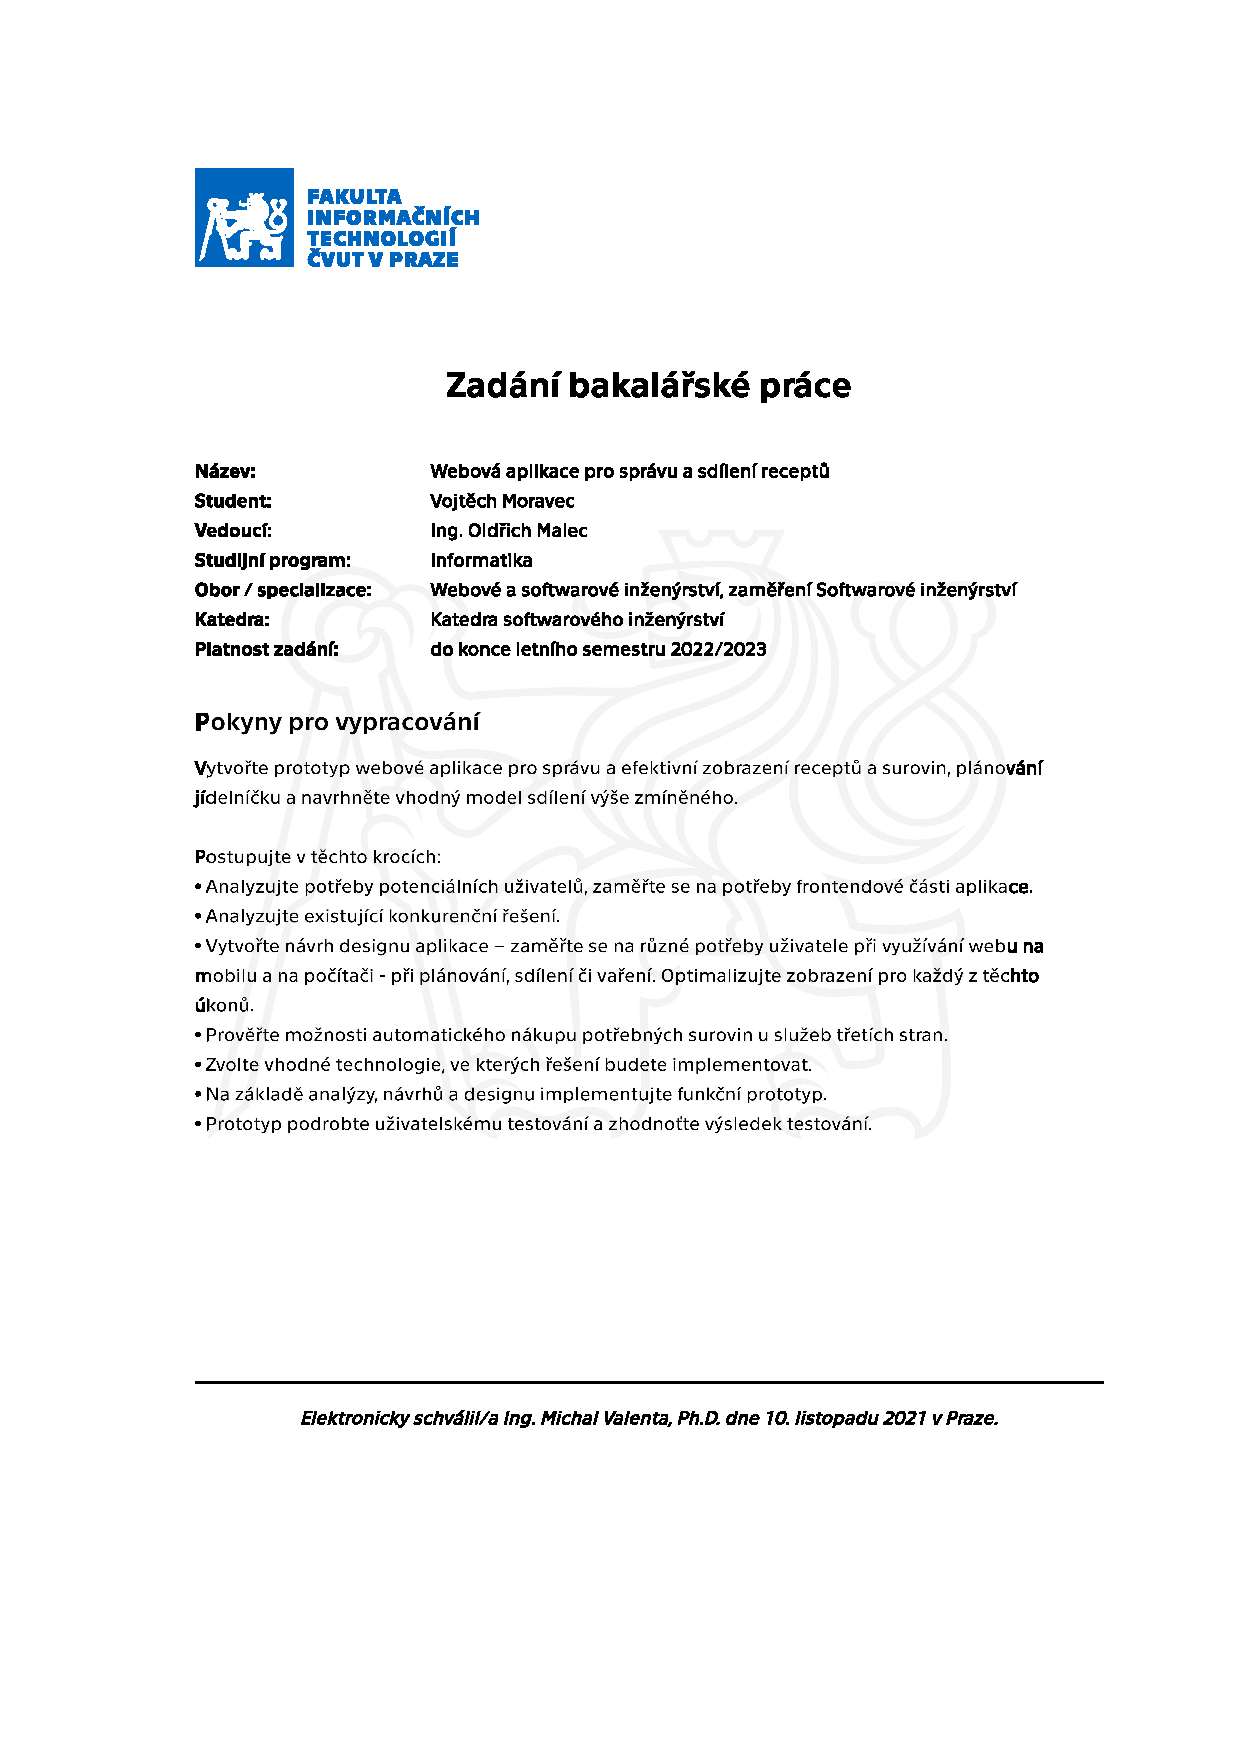
\includepdf{pdf/assignment-include.pdf} % replace that file with your thesis assignment provided by study office

\thispagestyle{empty}\cleardoublepage\maketitle % do not remove these three commands

\imprintpage % do not remove this command

\tableofcontents % do not remove this command
%%%%%%%%%%%%%%%%%%%%%%
% list of other contents: figures, tables, code listings, algorithms, etc.
% add/remove commands accordingly
%%%%%%%%%%%%%%%%%%%%%%
\listoffigures % list of figures
\begingroup
\let\clearpage\relax
\listoftables % list of tables
%\lstlistoflistings % list of source code listings generated by the listings package TODO: Minted switch
\listoflistings % list of source code listings generated by the minted package
\endgroup
%%%%%%%%%%%%%%%%%%%%%%
% list of other contents END
%%%%%%%%%%%%%%%%%%%%%%

%%%%%%%%%%%%%%%%%%%
% ACKNOWLEDGMENT
% FILL IN / MODIFY
% This is a place to thank people for helping you. It is common to thank your supervisor.
%%%%%%%%%%%%%%%%%%%
\begin{acknowledgmentpage}
	Chtěl bych poděkovat především sit amet, consectetuer adipiscing elit. Curabitur sagittis hendrerit ante. Class aptent taciti sociosqu ad litora torquent per conubia nostra, per inceptos hymenaeos. Cras pede libero, dapibus nec, pretium sit amet, tempor quis. Sed vel lectus. Donec odio tempus molestie, porttitor ut, iaculis quis, sem. Suspendisse sagittis ultrices augue.
\end{acknowledgmentpage}
%%%%%%%%%%%%%%%%%%%
% ACKNOWLEDGMENT END
%%%%%%%%%%%%%%%%%%%


%%%%%%%%%%%%%%%%%%%
% DECLARATION
% FILL IN / MODIFY
%%%%%%%%%%%%%%%%%%%
% INSTRUCTIONS
% ENG: choose one of approved texts of the declaration. DO NOT CREATE YOUR OWN. Find the approved texts at https://courses.fit.cvut.cz/SFE/download/index.html#_documents (document Declaration for FT in English)
% CZE/SLO: Vyberte jedno z fakultou schvalenych prohlaseni. NEVKLADEJTE VLASTNI TEXT. Schvalena prohlaseni najdete zde: https://courses.fit.cvut.cz/SZZ/dokumenty/index.html#_dokumenty (prohlášení do ZP)
\begin{declarationpage}
    Prohlašuji, že jsem předloženou práci vypracoval samostatně a že jsem uvedl veškeré
    použité informační zdroje v souladu s Metodickým pokynem o dodržování etických
    principů při přípravě vysokoškolských závěrečných prací.

    Beru na vědomí, že se na moji práci vztahují práva a povinnosti vyplývající ze zákona
    č. 121/2000 Sb., autorského zákona, ve znění pozdějších předpisů. V souladu s ust.
    § 2373 odst. 2 zákona č. 89/2012 Sb., občanský zákoník, ve znění pozdějších předpisů,
    tímto uděluji nevýhradní oprávnění (licenci) k užití této mojí práce, a to včetně všech
    počítačových programů, jež jsou její součástí či přílohou a veškeré jejich
    dokumentace (dále souhrnně jen „Dílo“), a to všem osobám, které si přejí Dílo užít.
    Tyto osoby jsou oprávněny Dílo užít jakýmkoli způsobem, který nesnižuje hodnotu
    Díla, avšak pouze k nevýdělečným účelům. Toto oprávnění je časově, teritoriálně
    i množstevně neomezené.
\end{declarationpage}
%%%%%%%%%%%%%%%%%%%
% DECLARATION END
%%%%%%%%%%%%%%%%%%%

\printabstractpage % do not remove this command

%%%%%%%%%%%%%%%%%%%
% SUMMARY
% FILL IN / MODIFY
% OR REMOVE ENTIRELY (upon agreement with your supervisor)
% (appropriate to remove in most theses)
%%%%%%%%%%%%%%%%%%%
\begin{summarypage}
\section*{Summary section}

\lipsum[1][1-8]

\section*{Summary section}

\lipsum[2][1-6]

\section*{Summary section}

\lipsum[3]

\section*{Summary section}

\lipsum[2]

\section*{Summary section}

\lipsum[1][1-8] Lorem lorem lorem.
\end{summarypage}
%%%%%%%%%%%%%%%%%%%
% SUMMARY END
%%%%%%%%%%%%%%%%%%%

%%%%%%%%%%%%%%%%%%%
% ABBREVIATIONS
% FILL IN / MODIFY
% OR REMOVE ENTIRELY
% List the abbreviations in lexicography order.
%%%%%%%%%%%%%%%%%%%
%! Author = vojmo
%! Date = 15.11.2021

\chapter{Seznam zkratek}

\begin{tabular}{rl}
    API & Application Programming Interface \\
    SQL & Structured Query Language \\
    NoSQL & Not Only SQL \\
    JSON & JavaScript Object Notation \\
    FE & Frontend \\
    NPM & Node Package Manager \\
    CLI & Command Line Interface \\
    YML & Yaml Ain't Markup Language \\
    JS & JavaScript \\
    PWA & Progressive Web App \\
    CSS & Cascading Style Sheets \\
\end{tabular}

%! Author = vojmo
%! Date = 15.11.2021

\chapter{Slovník}

\begin{tabular}{rl}
    Frontend & Část aplikace, kterou vidí uživatel a reaguje s ní \\
    Mesh gradient & Doplnit překlad \\ % TODO
    Drag and drop & Doplnit překlad \\ % TODO
    Firestore & Doplnit překlad \\ % TODO
    Firebase & Doplnit překlad \\ % TODO
    Cloud Storage & Doplnit překlad \\ % TODO
    Deploy & Doplnit překlad \\ % TODO
    Build & Doplnit překlad \\ % TODO
    Navigation Guard & Doplnit překlad \\ % TODO
    Prop & Doplnit překlad \\ % TODO
    Pop-up & Doplnit překlad \\ % TODO
    Sign-in provider & Doplnit překlad \\ % TODO
    Local storage & Doplnit překlad \\ % TODO
    Serverless & Doplnit překlad \\ % TODO
    Service workers & Doplnit překlad \\ % TODO
    Manifest & Doplnit překlad \\ % TODO
    Budget & Doplnit překlad \\ % TODO
\end{tabular}

%%%%%%%%%%%%%%%%%%%
% ABBREVIATIONS END
%%%%%%%%%%%%%%%%%%%

\mainmatter\mainmatterinit % do not remove these two commands

%%%%%%%%%%%%%%%%%%%
% THE THESIS
% MODIFY ANYTHING BELOW THIS LINE
%%%%%%%%%%%%%%%%%%%

%! Author = Vojta
%! Date = 21.10.2021

\chapter{Úvod}

Vaření se týká spousty lidí. Mladší generace k tomu používá recepty, které jsou dostupné na internetu. Recepty, které najdou
a které se jim osvědčí, jsou často na jiných stránkách a správa těchto receptů se stává nereálná. Na druhou stranu na nejznámějších
portálech není možné si recepty ukládat soukromně a tak spoustu starších lidí nevyužije možnosti digitalizace jejich receptů.
Většina z nich si totiž uchovává své recepty napsané na listech papíru, což ale v dnešní době již není praktické řešení. Už jen kvůli
sdílení receptu s někým, kdo si ho vyžádá, což je celkem běžná záležitost.

Výsledek této práce bude moci použít široká veřejnost -- každý kdo vaří podle receptů. Aplikace jim pomůže s jednoduchým
zadání receptů do sbírky, kde mohou mít všechny recepty na jednom místě. Dále budou moci uživatelé využít plánovače, kam
lze zanést již přidané recepty či počet porcí. Pokud nejsou zvyklí plánovat a spíše řeší věci na poslední chvíli, bude
pro ně připraven rychlý návrh receptu. V neposlední řadě bude jednoduché své recepty sdílet s ostatními uživateli.

V práci popisuji proces vývoje webové aplikace od analýzy přes návrh až po implementaci. Zaměřím se hlavně na frontend v
javascriptovém frameworku Vue.js, ale provedu čtenáře i backendovou částí, která je tvořena pomocí nástrojem Firebase od
společnosti Google. Začnu sběrem informací od potencionálních uživatelů, pomocí kterých sestavím funkční a nefunkční požadavky.
Poté zanalyzuji konkurenční řešení a popíšu jejich plusy či nevýhody. Poté představím technologie, které jsem si vybral pro
vývoj. Dále navrhnu uživatelské rozhraní, grafické prvky či datovou strukturu aplikace. Na základě předchozích kapitol implementuji
aplikaci a zmíním problémy, se kterými jsem se při vývoji setkal. Sestavím test pro uživatele a zhodnotím jeho výsledky.
Na závěr zmíním funkce které jsem nestihl implementovat či rozšíření, která by se v budoucnosti hodila.

Téma mě zaujalo, protože si myslím, že nabízí spoustu míst, pro učení se nových věcí. Také jsem nenašel žádnou alternativu,
která by nabízela všechny funkce, které moje řešení poskytuje.

\chapter{Cíl}
% TODO: Vylepšit
Cílem této bakalářské práce je vytvořit prototyp webové aplikace pro správu receptů. Dále je nutné prozkoumat možnosti
zjednodušení nákupu surovin či plánování vaření jídel.

Nejdříve zanalyzuji potřeby potenciálních uživatelů, kde se pokusím zjistit, které všechny funkce by ocenili. Poté se
zaměřím na existující řešení, která porovnám s mým řešením a popíšu vylepšení.

Dále vytvořím návrh designu aplikace -- wireframy, které zachycují zároveň, jak aplikace vypadá. Důraz kladu na rozdíly
mezi použitím na mobilu a počítači.

Na základě analýzy a návrhu vyberu technologie, které použiju pro implementaci funkčního prototypu.

Na konec podrobím aplikaci uživatelskému testování a zhodnotím jeho výsledky.

%! Author = vojmo
%! Date = 29.01.2022

\chapter{Analýza}

\section{Kvalitativní průzkum}

%TODO: Popsat více?
Nejprve bylo potřeba zjistit, co by potenciální uživatelé aplikace ocenili, tedy získat od nich požadavky.
Zvolil jsem kvalitativní průzkum, který se narozdíl od kvantitativního zaměřuje na malou skupinu respondentů.
Pro získání odpovědí jsem si připravil sadu otevřených otázek, kterých jsem se držel při rozhovoru. Hovory byly
uskutečněny online a každy trval mezi dvaceti minutami a jednou hodinou.

Na začátek jsem představil aplikaci a poté jsem se ptal na lehčí otázky, které odlehčili situaci. Postupně jsem se
propracoval k specifičtějším otázkám. Po několika rozhovorech se již odpovědi začaly opakovat a tak jsem už další
neprováděl.

\subsection{Seznam otázek}
\begin{itemize}
    \item Jak často vaříš?
    \item Co ti na vaření vadí a co tě naopak baví?
    \item Jaké recepty používáš?
    \item Používáš online recepty (co ti na nich vadí), pokud ano, na mobilu nebo na PC?
    \item Jak vypadají recepty, které máš napsané na papíru?
    \item Máš radši vlastní recepty nebo hledáš inspiraci jinde?
    \item Upravuješ si cizí recepty, popřípadě jak?
    \item Co si myslíš o možnosti vytvoření vlastní online kolekce receptů, které máš na papíře?
    \item Uvítal bys, kdyby se importování receptů provádělo pomocí telefonu?
    \item Je něco, co by vaření podle online receptů usnadnilo?
    \item Jak často nakupuješ?
    \item Kolik času nakupováním strávíš?
    \item Použil jsi někdy rohlik.cz nebo podobné služby?
\end{itemize}

Všechny rozhovory byly vedeny v rozmezí dvou týdnů a poté jsem z nich sestavil funkční a nefunkční požadavky.

\section{Funkční požadavky}


\begin{itemize}
    \item F1: Správa receptů

    Pro uživatele je důležité udržovat své recepty aktuální. Je tedy nutné implementovat rozhraní, které umožní pracovat s
    přidanými recepty.
    \item F2: Sdílení receptů

    Narozdíl od ostatních služeb, které jsou popsány dále v textu, by tato měla poskytovat sdílení mezi uživateli. Na to se pojí i
    viditelnost receptů, tedy všechny nebudou veřejné, ale bude možné je přidat jako soukromé či neveřejné.
    \item F3: Objednávky přes služby typu rohlik.cz

    Převážně mladší generace dnes hojně využívá služeb na rozvoz nákupu. Je tedy potřeba přidat zjednodušený přesun potřebných
    surovin do nákupních košíků v těchto službách, a tak zefektivnit čas nákupu.
    \item F4: Plánovač

    Pro mnoho lidí je důležité naplánovat si kdy mají čas si jídlo uvařit a naopak kdy by ho potřebovali mít již hotové. Pro bude v
    aplikaci plánovač, kde bude uživatel moci sledovat, kdy ho čeká co uvařit.
    \item F5: Správa spíže

    Tento požadavek souvisí s těmi předchozími, tedy hlavně ulehčí uživateli nákup surovin a plánování vaření. Pokud uživatel nebude chtít
    kontrolovat jaké suroviny má doma, funkci nebude muset využít.
    \item F6: Možnost ankety kolem jídelníčku

    Spíše než v běžném životě by se anketa dala využít například při výletu s kamarády či soustředění s týmem nebo kapelou. Uživatelé
    by měli možnost hlasovat, v jaký den a jaké jídlo by chtěli.
\end{itemize}

\section{Nefunkční požadavky}

\begin{itemize}
    \item U1: Dostupné jako webová aplikace

    Vzhledem k potřebě mít aplikaci dostupnou jak pro mobily, tak pro počítač, je webová aplikace nejflexibilnější řešení.
    \item P1: Systém pro jednotky uživatelů

    Aplikaci nebude využívat mnoho uživatelů, ale je nutné myslet na budoucí rozšíření.
    \item S1: Serverless s možností připojení na speciální API v budoucnu

    Prozatím se pro backendovou část využije \emph{serverless} řešení. Pokud by tato alternativa v budoucnu neposkytovala dostatečné
    funkce nebo se nevyplatila finančně, je možné přejít na jiný backend.
\end{itemize}

\begin{figure}[H]
    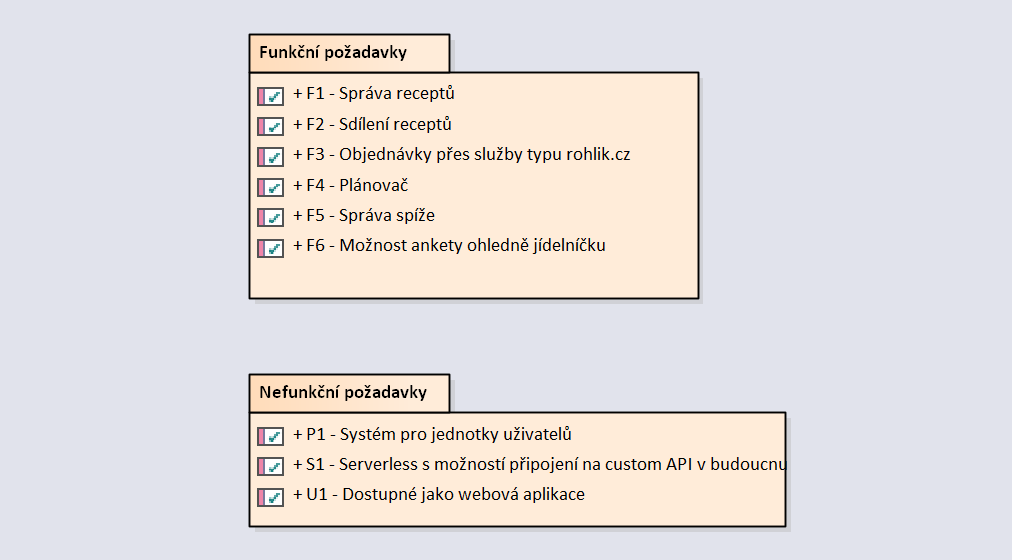
\includegraphics[width=\textwidth]{images/pozadavky}
    \caption{Model požadavků} \label{picture:recipeo:pozadavky}
\end{figure}

\section{Existující řešení}

Porovnal jsem nejpoužívanější české portály s recepty. Některé z nich nabízejí další obsah jako například blog či magazín.

\subsection{Vareni.cz}

Na vareni.cz~\cite{VareniCZ} se nachází několik reklam, které jsou velké a rušivé. Není zde možné si přidat soukromý recept a sdílet ho
pouze s vybranými uživateli. Celkový koncept přidání receptu je pouze veřejný, není tedy možné si zde vytvořit sbírku
oblíbených receptů z různých portálů. Vyhledávání je možné podle názvu, ingrediencí či různých parametrů jako je druh jídla
nebo národní kuchyně. Recepty mají hodnocení od jedné do pěti hvězdiček.

Na stránce konkrétního receptu je shrnutí nejdůležitějších vlastností, tedy název, krátký popis, hodnocení a čas vaření.
Také v hlavičce kolují různé komentáře. Výhodou jsou návrhy podobných receptů. Naopak velmi špatné je rozložení seznamu ingrediencí
a postupu přípravy. Tato část je velmi nepřehledná a je nerozeznatelné kde recept končí a začínají jiné recepty.

Jsou zde kuchařky, ale než že by byly tématické nebo měli společného autora, přišlo mi, že se jedná se o náhodnou kolekci receptů,
kde je jich často více než tisíc.

Celkem hezký nápad jsou fotorecepty. Uživatele provedou celým vařením pomocí kroků, přičemž u každého je fotodokumentace jak daný krok
provést.

\begin{figure}[H]
    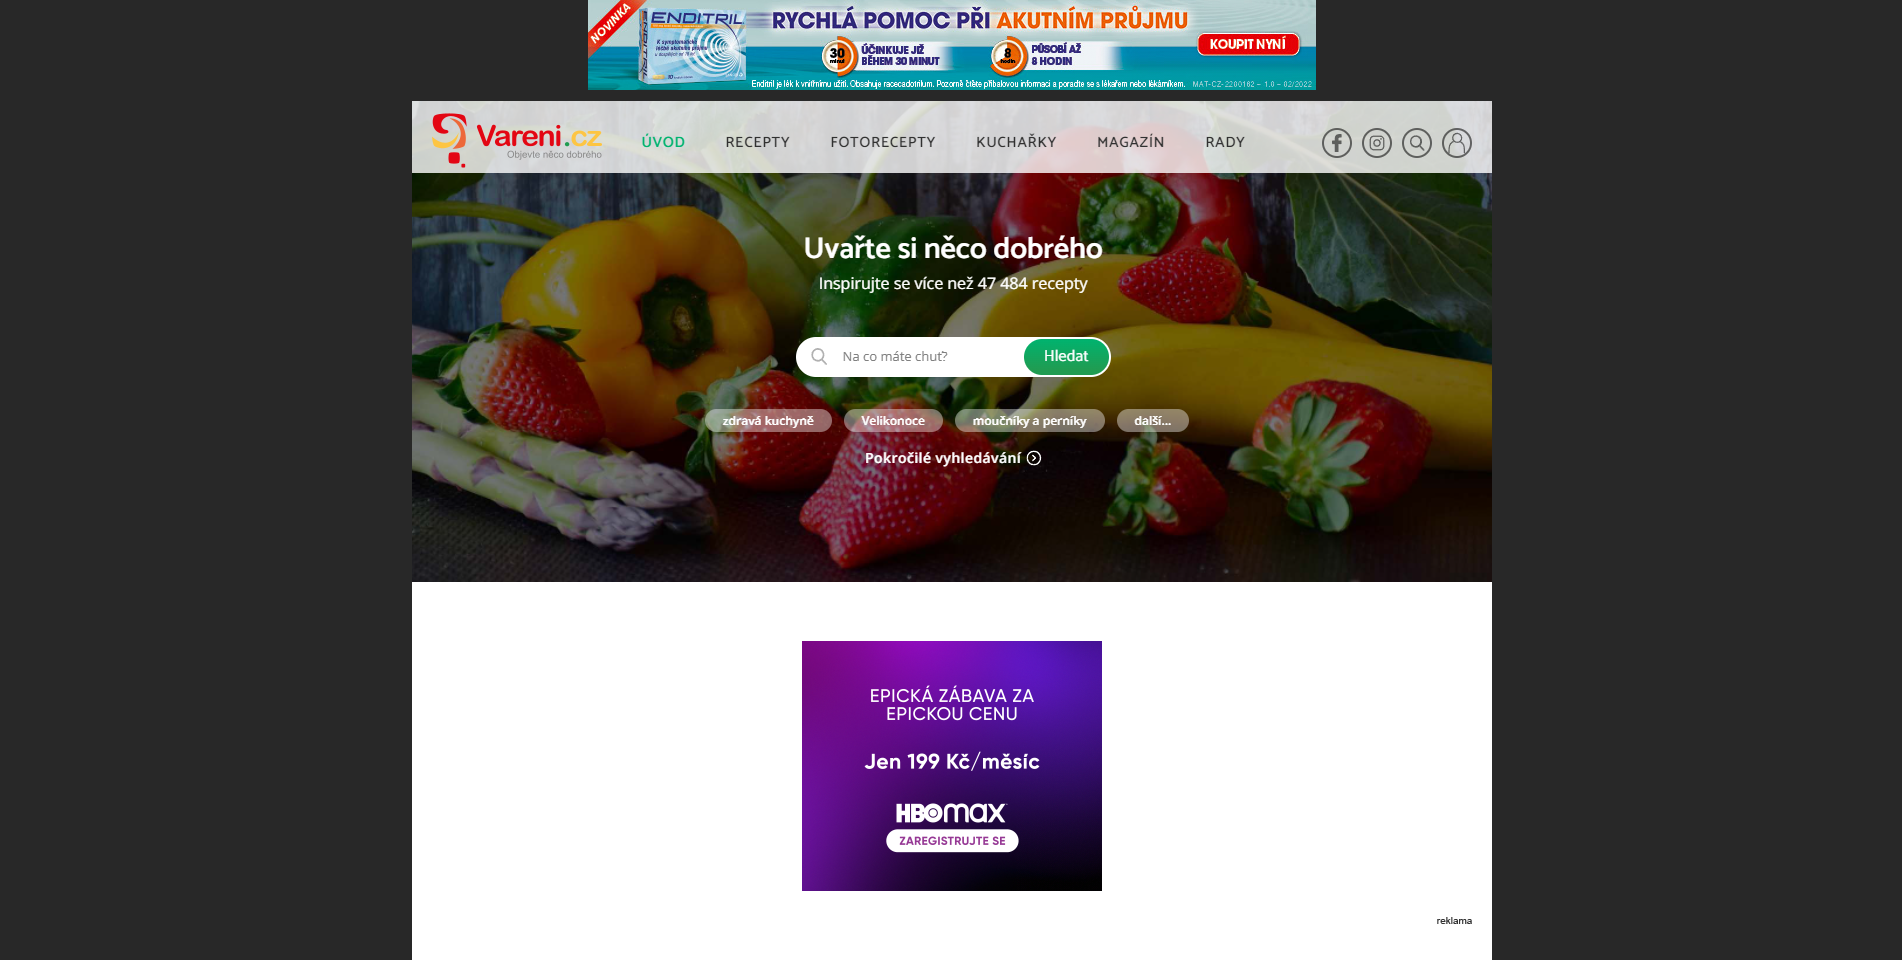
\includegraphics[width=\textwidth]{images/varenicz-uvodni-stranka}
    \caption{Hlavní stránka vareni.cz} \label{picture:varenicz:uvodni-stranka}
\end{figure}

\subsection{Toprecepty.cz}

Na tomto portálu~\cite{TopreceptyCZ} byla bohužel nefunkční registrace, takže jsem nemohl nahlédnout na funkce poskytované přihlášeným
uživatelům. Opět zde byla přítomna velká reklama, která zabírala většinu stránky. Jinak byl web navrhnut přehledně,
ale narazil jsem na několik nefunkčních prvků na mobilním zobrazení. Zhodnotit přidání receptů a jak funguje jejich
sdílení zhodnotit nemohu, kvůli výše zmíněným problémům. Našel jsem funkci podobnou doporučování receptů, avšak se
pravděpodobně jedná o náhodné doporučení, které nemá nic společného s tím co má uživatel rád. Dále je na webu dostupný
online magazín, kde jsou různé články týkající se gastronomie.

\begin{figure}[H]
    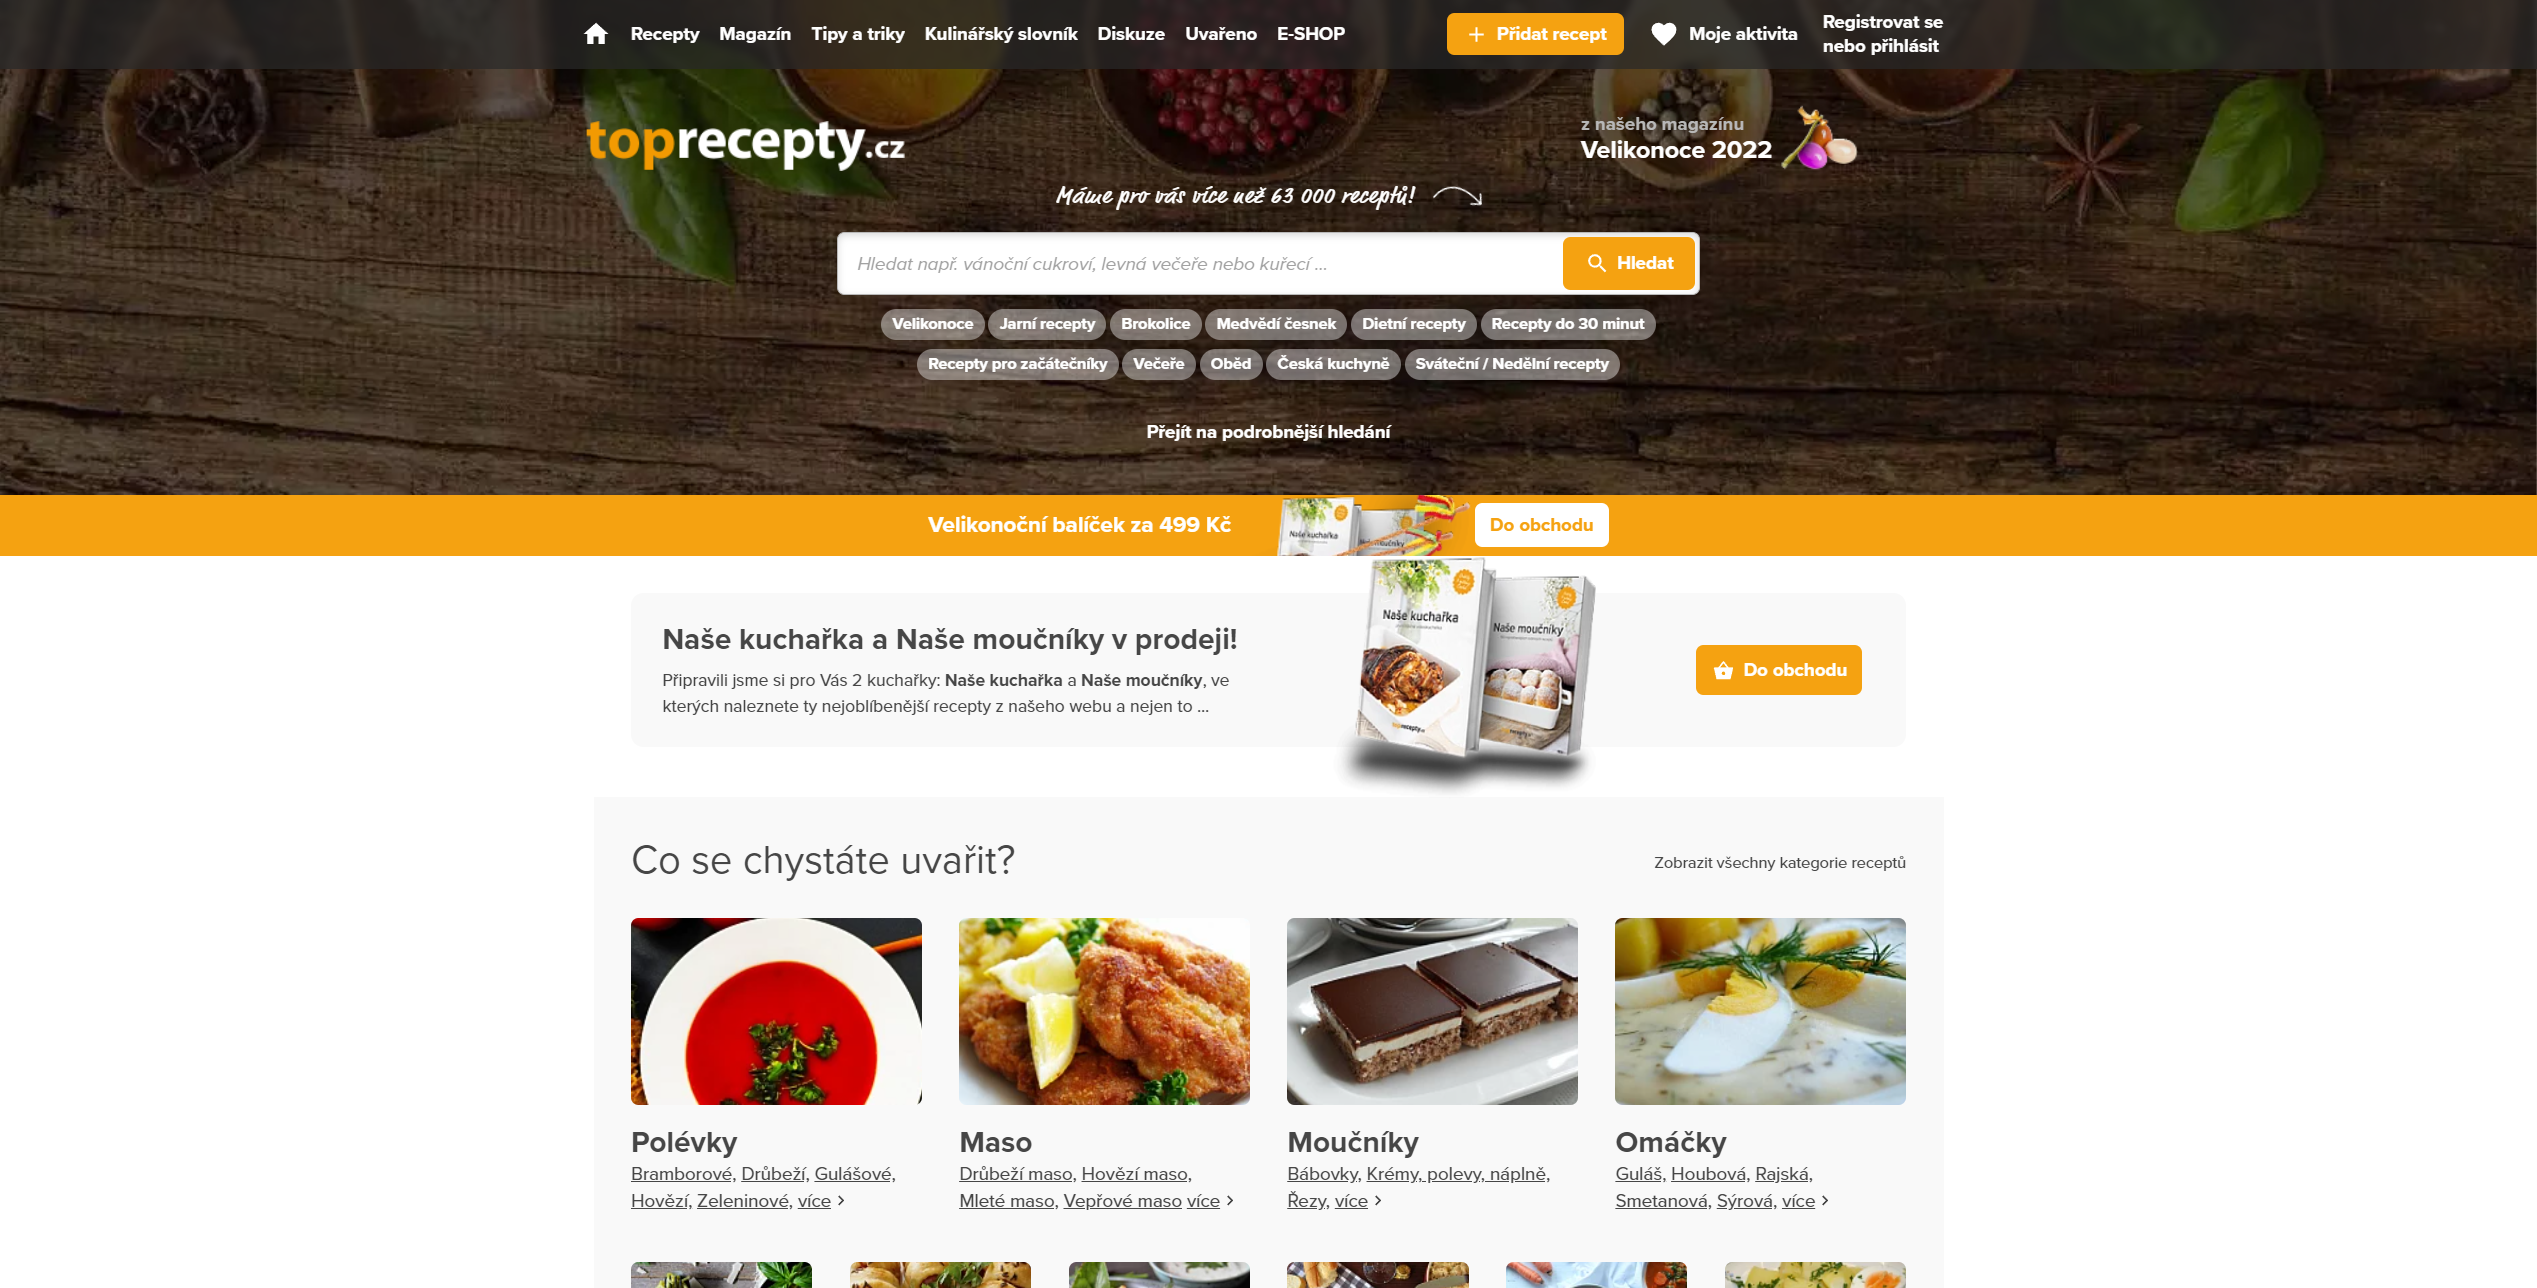
\includegraphics[width=\textwidth]{images/topreceptycz-uvodni-stranka}
    \caption{Hlavní stránka toprecepty.cz} \label{picture:topreceptycz:uvodni-stranka}
\end{figure}

\subsection{Recepty.cz}

I třetí zástupce~\cite{ReceptyCZ} existujících řešení používá reklamu přes celou stránku okolo jejího obsahu. Podobně jako toprecepty.cz
je zde magazín obsahující příspěvky na spoustu témat o vaření. U přidání receptu nebylo napsané, co se s receptem stane,
zda bude veřejný nebo se zobrazí pouze mě. Po kliknutí na tlačítko \uv{Uložit recept}, se zobrazila stránka s nadpisem
\uv{Recept čeká na schválení}. Nebylo tedy opět možné soukromé použití.

Zobrazení receptu je podobné tomu na vareni.cz, ale přijde mi více přehledné. U kroků se zobrazují rady, které ale
nemají s daným krokem nic společného, spíše odkazují na náhodné články či recepty.

\begin{figure}[H]
    \includegraphics[width=\textwidth]{images/receptycz-uvodni-stranka}
    \caption{Hlavní stránka recepty.cz} \label{picture:receptycz:uvodni-stranka}
\end{figure}

\subsection{Závěr}

Existující řešení na vyhledávání receptů nabízejí pouze veřejné recepty a mají spoustu reklam. Moje řešení bude poskytovat
možnost soukromé sbírky receptů a jejich sdílení s vybranými uživateli či pomocí odkazu.

Sestavil jsem tabulku s hodnocením od jedné do pěti, stejné jako se používá ve škole. Každý aspekt jsem ohodnotil pro všechny
stránky, které jsem zahrnul v porovnání a přidal jsem skóre, které je v souladu s parametry mojí aplikace.

\begin{table}[H]\centering
    \caption{~Porovnání konkurenčních řešení}\label{tab:recipeo:konkurencni-reseni}
    \begin{tabular}{l|c|c|c|c}
        Typ		    & vareni.cz & toprecepty.cz & recepty.cz & recipeo.cz \tabularnewline \hline
        Reklamy		& 4		    & 2	            & 3          & 1          \tabularnewline \hline
        Zobrazení receptu	    & 3		    & 2	            & 3          & 1          \tabularnewline \hline
        Doporučování receptů	    & 2		    & 2	            & 2          & 3          \tabularnewline \hline
        Model sdílení	    & 4		    & 4	            & 4          & 2          \tabularnewline \hline
        Zjednodušení nákupu	    & 4		    & 3	            & 2          & 1          \tabularnewline
    \end{tabular}
\end{table}

\section{Nákup surovin}

Vedoucí práce již dříve používal aplikaci Zdravý stůl~\cite{ZdravyStul}. Tam bylo možné si jídlo objednat přes rohlik.cz (vložit do košíku).
Tudíž jsme chtěli tuto funkcionalitu zachovat a přidat možnosti jako například vytvoření objednávky u konkurence - kosik.cz
či zobrazení interaktivního nákupního listu.

\subsection{Komunikace s Rohlíkem a Košíkem}
Nejdříve jsem se rozhodl kontaktovat Rohlík. Po pár vyměněných e-mailech jsem obdržel celou dokumentaci k jejich API,
které nám otevřelo spoutu možností i do budoucna. Například bychom mohli sledovat, jaké suroviny jsou právě ve slevě a
podle toho doporučovat jídla.

Od Košíku jsme dostali pozvání na schůzku, kde jsme si mohli prohlédnout i jejich kanceláře. Na schůzce jsme hned na začátku
zjistili, že API pro partnery narozdíl od Rohlíku ještě dostupné není (Rohlík na API pro partnery také teprve pracuje,
ale zatím jsme dostali přístup k API pro jejich aplikaci), ale už na něm pracují. Plánované období vydání je
první kvartál roku 2022. Pro jeho využití je však potřeba OAuth server, který zatím není dostupný. % TODO: Zjistit v lednu.
Jako alternativu jsme dohromady vymysleli link na přidání surovin přímo do košíku, ze kterého nakonec sešlo, protože jsme
poté objevili funkci \uv{Nákupní lístek}, kterou bychom mohli využít. Odeslali bychom seznam surovin a uživatel by si je poté
mohl vybrat přímo z nabídky na Košíku. Nakonec jsme zjistili, že by se Košíku hodilo rozrůst sbírku receptů a bylo by možné
pro uživatele naší aplikace nabínout jejich recepty Košíku, který by je následně odkoupil.

%! Author = Vojta
%! Date = 21.10.2021

\chapter{Technologie}

\section{Výběr}
Vzhledem k tomu, že aplikace byla původně zamýšlena jako osobní projekt, který by si následně spravoval sám vedoucí a já
jsem měl zkušenosti pouze s frameworkem Vue.js, hlavní technologie, okolo které se projekt postaví, byla předem daná. Poté
jsem postupně vybíral další součásti, které bychom mohli využít. Velkou výhodou bylo, že právě vedoucí práce má s většinou
z těchto knihoven či pluginů zkušenosti, a tak když se mi něco nedařilo, mohl jsem se na něj obrátit.

\section{Vue.js}
Vue je progresivní JavaScriptový framework, který narozdíl od konkurenčních řešení (React, Angular) nezaštiťuje žádná velká
korporace, ale je vyvíjen komunitou.\cite{VueJS} Zvolil jsem verzi 3, protože je to lepší řešení do budoucna, než později aktualizovat
celou aplikaci z verze 2. V pozdější fázi vývoje se ale ukázalo, že pro verzi 3 nebyla plně dokončena hlavní knihovna, kterou jsem chtěl využít.
Musel jsem tak ponížit verze všech závislostí a přejít tak na verzi 2.

\section{Vuetify}
Vuetify je knihovna implementující různé komponenty, které je možné použít při tvorbě uživatelského rozhraní. Kromě toho
usnadňuje práci s rozložením na stránce, přizpůsobením barevného téma, ikonami atd. Další výhodou jsou týdenní aktualizace
momentální verze, které přidávají nové funkce a opravují nalezené chyby.\cite{VuetifyWhy}
Bohužel tato knihovna nebyla v době vývoje plně dokončena a byla pouze v alpha verzi, tudíž spoustu věci nefungovalo jak by mělo.

\section{Vuex}
Knihovna Vuex~\cite{Vuex} se využívá pro uložení stavu aplikace. Je vhodné ji využít u dat, která jsou využívána na více místech a jejich
předávání skrz komponenty by bylo jinak složité.

Změna či přístup k stavu a všechny operace nad ním se řeší ve speciálním souboru, kde se Vuex inicializuje. K těmto operacím využijeme \emph{state, mutations, getters, actions a modules}.
\emph{State} označuje strukturu dat, tedy pokud potřebuji nějak zaznamenávat recepty, vytvořím zde pole či objekt a s ním dále pracuji. Pro to abych přidal recept využiji \emph{actions} v kombinaci s
\emph{mutations}. \emph{Actions} je obal funkcí, které můžu zavolat odkudkoliv z aplikace a ty provedou nějakou změnu nad daty. Například data stáhnou, aktualizují nebo nastaví hodnotu, kterou uživatel
zadá. Mutations poté vyvoláme pomocí funkce \mintinline{js}|commit|. Té předáme název mutace, která se má zavolat a tzv. \emph{payload}, tedy data, která chceme do stavu zapsat. Mutace již poté pouze zapíše
do stavu a nic dalšího by řešit neměla.

Pro získání stavu lze využít \emph{getters}. V těchto funkcích by také neměla být žádná další logika, ačkoliv se zde dá vytvořit drobné filtrování či řazení.
Když se aplikace rozroste a obsahuje mnoho dat, tak aby všechny tyto části byly přehledné, je možné vytvořit více modulů a spravovat data která mají něco společného
odděleně. Samotné moduly se pak naimportují do \emph{modules} a jsou přístupné v celé aplikaci.

\section{Vue i18n}
I18n~\cite{i18n} je rozšíření pro překlady, díky kterému je možné texty v aplikaci napsat v několika jazycích. Nejprve jsem tvořil aplikaci dvojjazyčně
v angličtině a čestině, ale nakonec jsem se rozhodl, že prozatím dává aplikace smysl pouze v češtině. Nicméně překlady jsem ponechal a v budoucnu
je možné je využít.

\section{Firebase}
Firebase~\cite{Firebase} je platforma pro vývoj aplikací. Nabízí spoustu produktů, které je možné využít a tím zjednodušit vývoj.
Dané produkty mohou mezi sebou komunikovat a reagovat na různé události. Firebase poskytuje multiplatformní SDK, což znamená, že je
možné vyvíjet v několika programovacích jazycích jako je Java, Kotlin, Swift, JavaScript nebo C++. V kombinaci s touto platformou je možné
využít další nástroje od společnosti Google, jako jsou Analytics, Google Ads a další. K tomu lze přidat rozšíření, které vyžadují jen základní
konfiguraci a propojí aplikaci s dalšími externími systémy, jako je Stripe~\cite{Stripe} či Algolia~\cite{Algolia}.

\subsection{Ceny}
Firebase má velikou výhodu v tom, že je zdarma, pokud uživatelé nevyčerpají určitý objem dat či přístupů k databázi. Tato kapacita se resetuje
denně nebo měsíčně, podle toho o jaký podsystém se jedná. V nabídce jsou dva plány. První \emph{Spark Plan} je úplně zadarmo, ale má určitá omezení.
Na druhou stranu \emph{Blaze Plan} má stejné limity a platí se pouze za jejich překročení. Tedy například pro databázi Firestore je zdarma padesát tisíc
čtení denně pro oba plány a pro \emph{Blaze Plan} poté stojí každých dalších sto tisíc čtení 1,40 Kč.~\cite{FirebasePricing}

\subsection{Firestore}
Cloud Firestore~\cite{Firestore} je NoSQL dokumentová databáze. Narozdíl od SQL databází, které se soustředí na snížení duplikace dat, se dokumentová
databáze zaměruje na časté aktualizace a změny. Největší rozdíl mezi těmito typy je způsob uložení dat. SQL reprezentuje data pomocí
tabulek s řádky a sloupci, dokumentová databáze má JSON dokumenty a jejich kolekce. To vede k flexibilnějšímu datovému modelu, rychlejším
dotazům a lehčímu vývoji pro vývojáře.~\cite{MongoDBNoSQL}

Firestore nabízí vlastní řešení bezpečnosti přes Firebase Rules, které více přiblížím v kapitole o implementaci pomocí ukázek.

\subsection{Storage}
Cloud Storage je uložiště, kam je možné ukládat různé soubory, které uživatelé poutřebují při používání aplikace. V mém případě to
budou fotografie jídel či surovin. Pro ukládání dat se používají takzvané \emph{Cloud Storage buckets}, což jsou pouze kontejnery,
které můžeme využít tak, aby data byla organizovaná~\cite{FirebaseBucket}. K tomu lze vytvořit vnitřní strukturu pomocí složek nebo
data oddělit podle jejich provázanosti do různých kontejnerů.

\subsection{Hosting}
Webová aplikace musí být někde dostupná, aby k ní uživatelé mohli přistoupit. K tomu lze v rámci Firebase využít \emph{Hosting}.
Ten nabízí rychlé SSD disky, na kterých web běží, SSL certifikáty pro vlastní domény zdarma, jednoduchý \emph{deploy} nebo náhledy
aplikace předtím než je nasazena na produkci.~\cite{FirebaseHosting}

\subsection{Functions}
Firebase Cloud Functions mají za úkol vývojářům ulehčit vývoj backendu tak, aby nemuseli řešit záležitosti okolo správy serverů.
Funkce, které na tomto systému běží mohou reagovat na širokou škálu událostí uvnitř Firebase produktů. Například pokud se do aplikace
přihlásí nový uživatel, může se spustit funkce, která mu odešle uvítací email. Jako programovací jazyk se pro psaní funkcí použivá Node.js.~\cite{FirebaseFunctions}

\section{Fulltextové vyhledávání}
Při práci s Firebase jsem zjistil, že při dotazování se na záznamy není možné filtrovat podle názvu
(abych byl přesný, možné to je, ale není to vhodné). Po zkoumání dokumentace, jsem našel stránku s doporučením pro
fulltextové hledání. V nabídce byla tři řešení.~\cite{FulltextSearch}

\begin{itemize}
    \item Elastic
    \item Algolia
    \item Typesense
\end{itemize}

Problém jsem řešil s vedoucím a přišli jsme na několik možných řešení sami. Stáhnout si data o všech receptech ve formátu
\emph{id:name} a poté filtrovat výsledky hledání na FE. Dále bychom mohli použít Firebase Cloud Functions, kde bychom
využili hashování. Nakonec jsem se ale rozhodl, že využiji jedno z nabízených řešení přímo Googlem.

Vybral jsem Algolii~\cite{Algolia}, kvůli dobré podpoře Vue a Firebase, nejmenší složitosti implementace a bezplatnému základnímu plánu.

Při vývoji jsem ale zjistil, že základní režim (tedy 10 000 čtení za měsíc) nejspíše stačit nebude. Nakonec jsem proto přešel na
frontendové vyhledávání. Všechna data jsem stáhnul při načtení aplikace a poté s nimi dál pracoval.

\section{Vue Router} % TODO: Více rozepsat
V aplikaci je potřeba mít navigaci. Ve Vue se používá Vue Router~\cite{VueRouter}, který umožní pohyb po různých stránkách.

\subsection{SPA}
SPA neboli \emph{single page application} je stránka, která využívá takové architektury, kde použitá technologie nejen kontroluje
vzhled stránky, ale i data a manipulaci s nimi a navigaci tím způsobem, že není nutné provádět obnovení stránky.\cite{VueSPA}

Pro demonstraci rozdílu mezi MPA a SPA jsem zvolil následující diagramy.

\begin{figure}[H]
    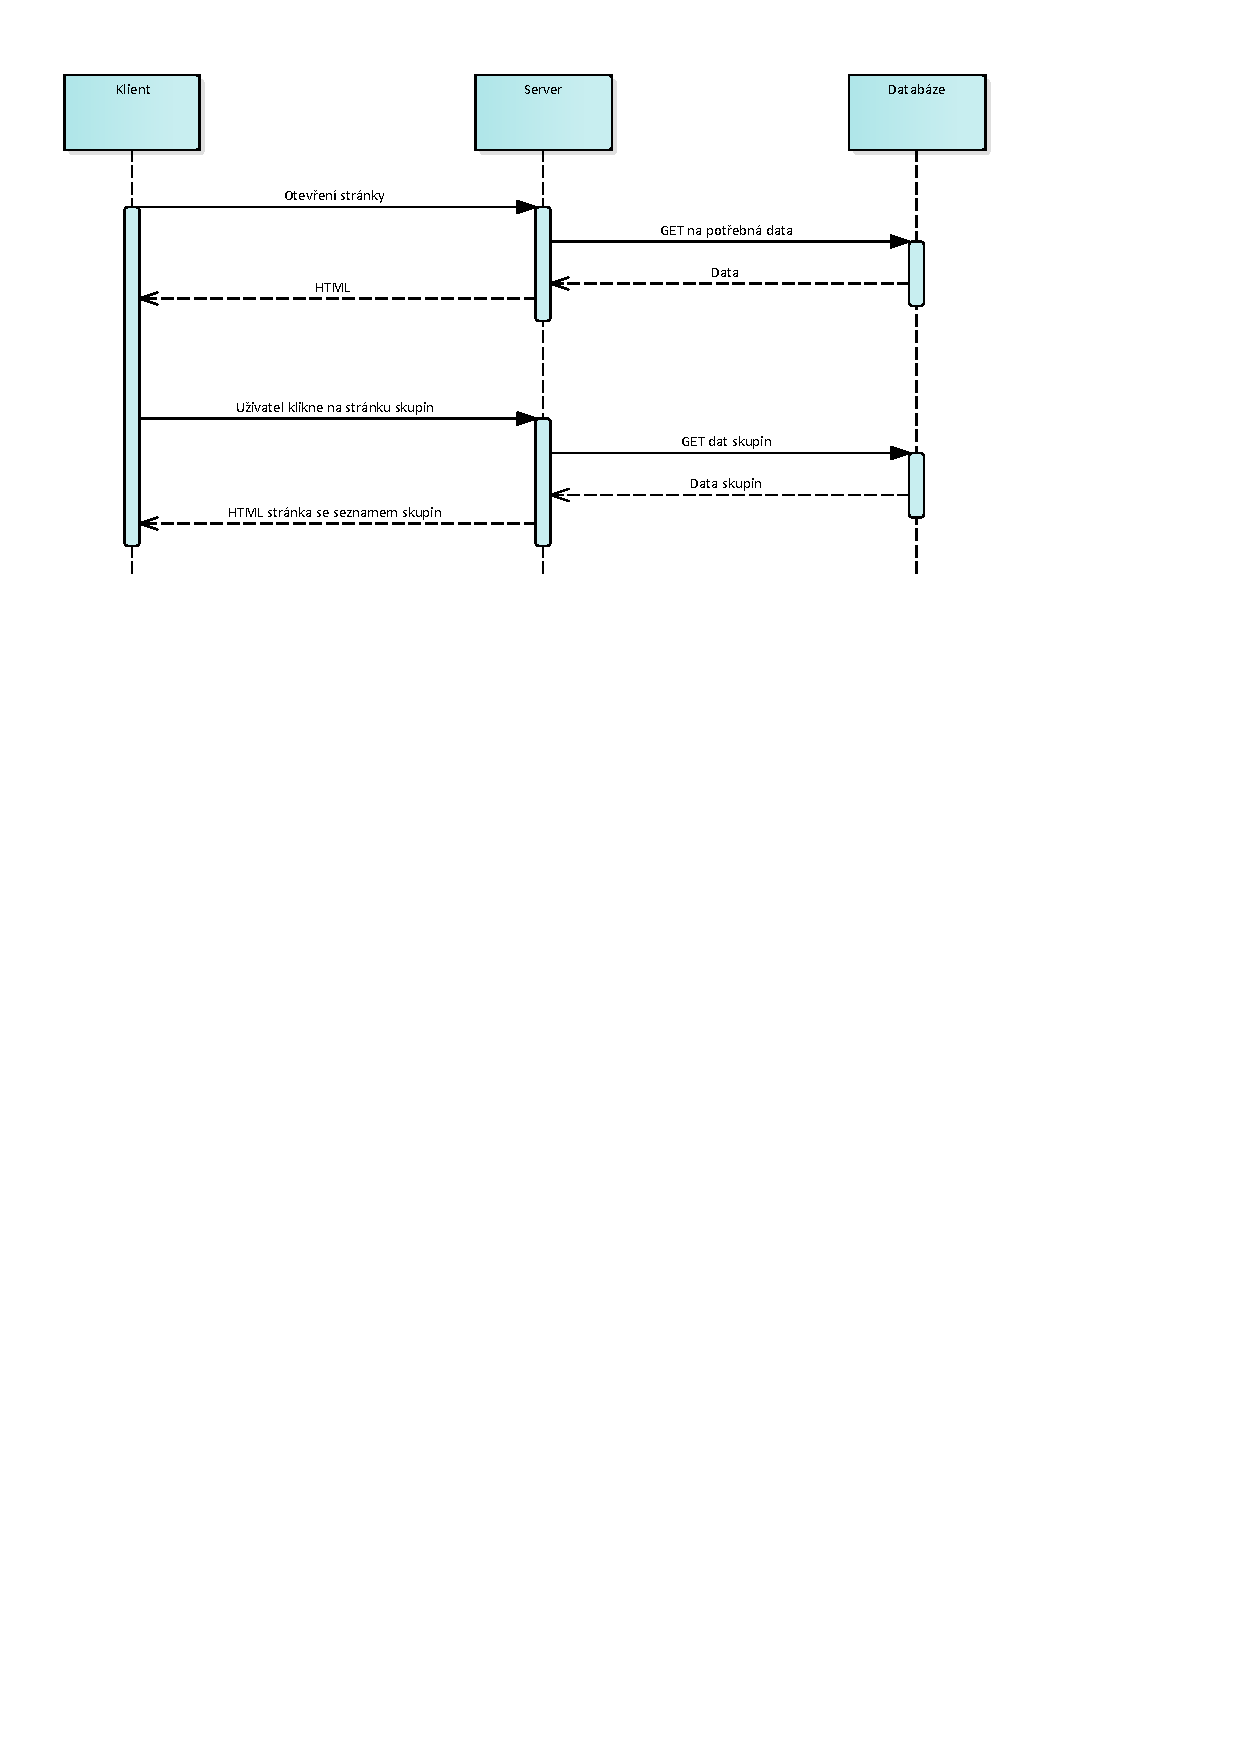
\includegraphics[width=\textwidth]{pdf/MPA-model}
    \caption{MPA Model} \label{picture:recipeo:mpa-model}
\end{figure}
\begin{figure}[H]
    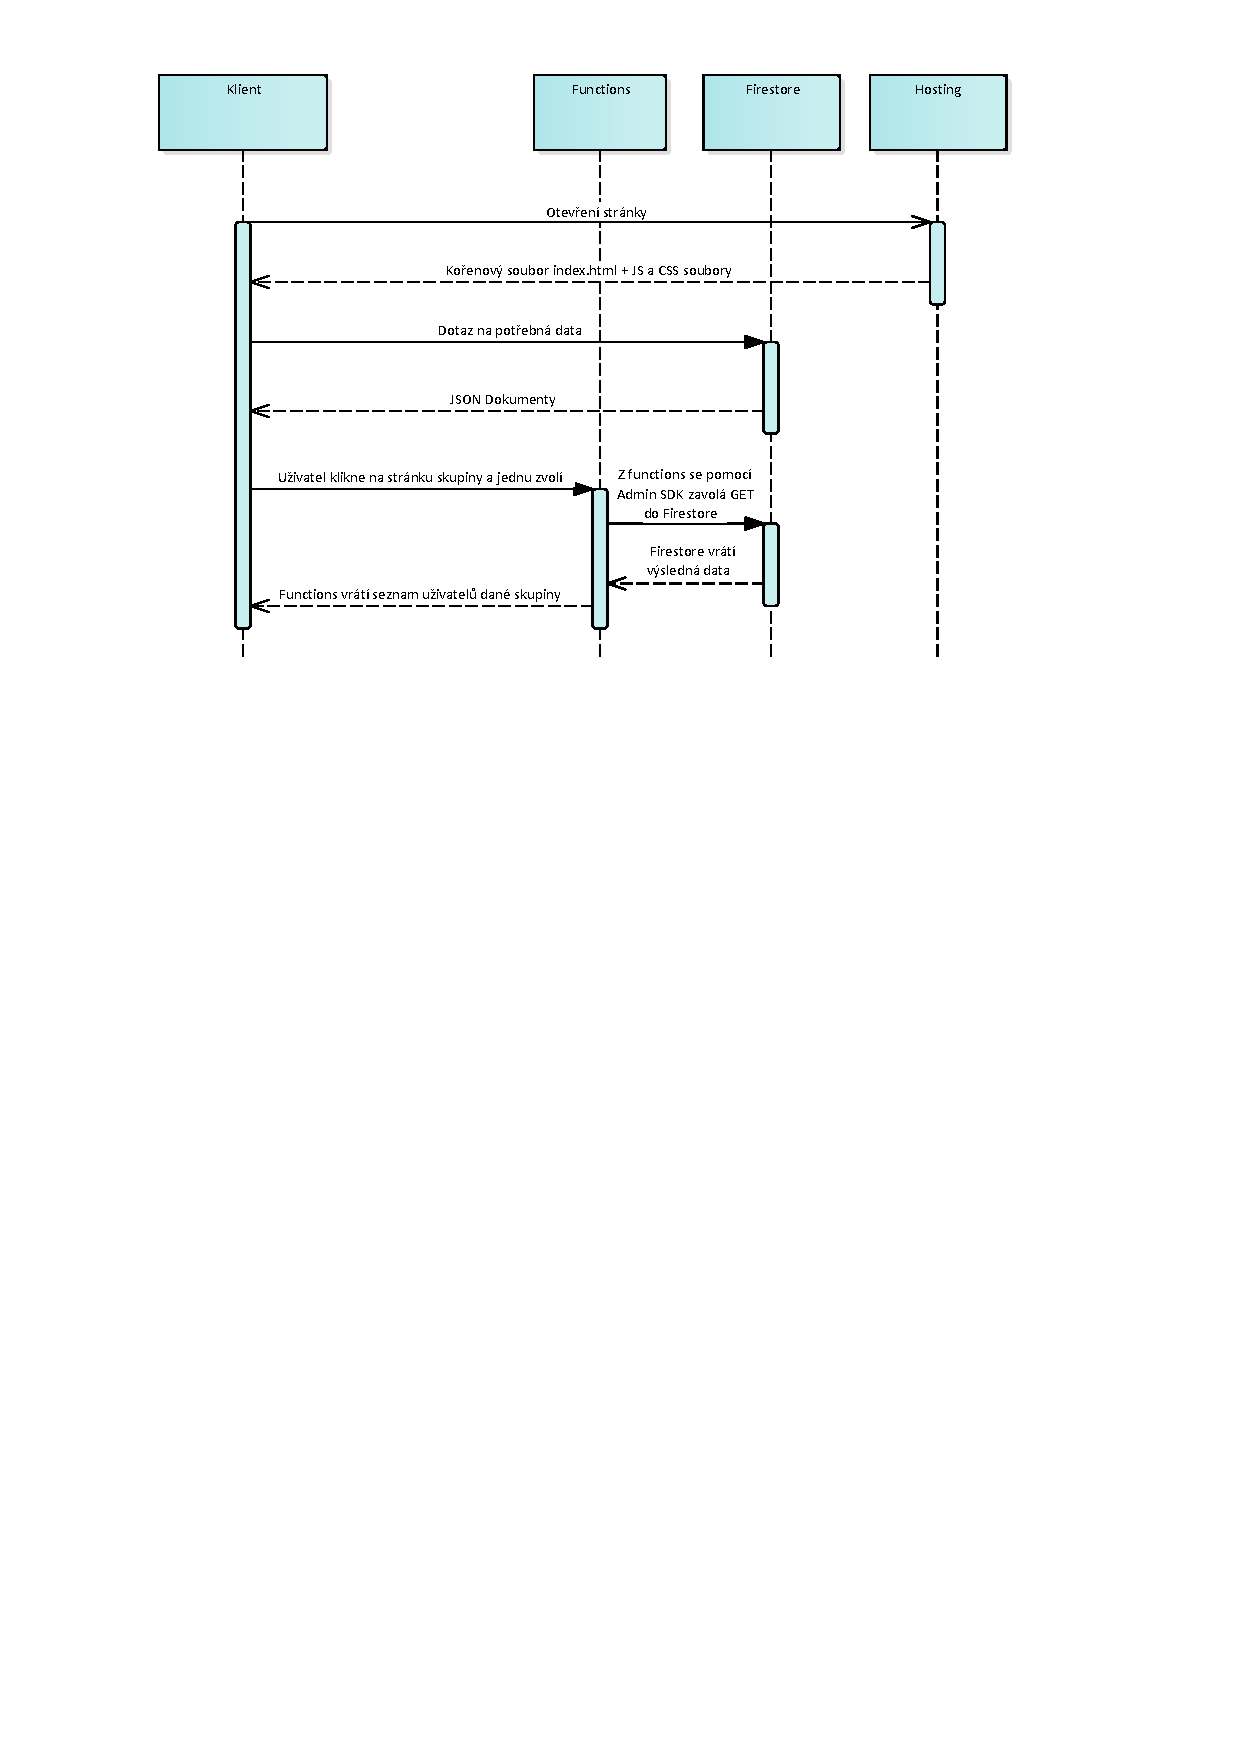
\includegraphics[width=\textwidth]{pdf/SPA-model}
    \caption{SPA Model} \label{picture:recipeo:spa-model}
\end{figure}

Jak je ve SPA diagramu vidět, některá data lze získat přímým přístupem do Firestore, ale jiná je nutné stáhnout z Functions.
Je to dané tím, že u některých dat není možné ošetřit jejich bezpečnost pomocí Firestore Rules a je tedy nutné k nim přistupovat
přes Functions, které má dostupné Admin SDK, tedy neomezený přístup k celé databázi. Data tak mohou být pro běžné uživatele nepřístupná,
ale pomocí volání cloudové funkce přímo z aplikace je možné je stáhnout. Také se dají data tímto způsobem předzpracovat, což může
být výhodné právě z hlediska bezpečnosti a k uživateli se tak nedostane nic co by nemělo.

\section{PWA}

Progresivní webová aplikace se snaží usnadnit vývoj standardních webových aplikací jako nativní aplikace pro mobilní telefony.
K tomu využívá \emph{service workers} a webové aplikační \emph{manifesty}. Aby se aplikace dala považovat za PWA, měla by
mít tyto vlastnosti~\cite{PWAAckee}.


\begin{itemize}
    \item Progresivní

    Je použitelná na starších prohlížečích s určitými omezeními, ale plně funkční na nejnovějších verzích prohlížečů.
    \item Responzivní

    Stránka je optimalizována pro všechny typy obrazovek (od nejmenších telefonů, přes notebooky až po velké PC monitory)
    \item Nezávislá na konektivitě

    Pomocí technologie \emph{service workers} je možné aplikaci využívat offline díky cachování
    \item App-like

    Aplikace vypadá jako nativní ačkoliv na pozadí je webová aplikace
    \item Aktuální

    Poskytují vždy aktuální verzi díky procesu update technologie \emph{service workers}
    \item Zabezpečená

    Výhradní použití HTTPS zamezí odposlouchávání či jiné manipulaci s přijímanými daty
    \item Znovuzapojení uživatele

    Je možné využít funkce push notifikace, která poté uživatele naláká zpět do aplikace \footnote{Tyto push notifikace z webového prohlížeče jsou již několik let běžnou
    záležitostí na systému Android, ale do iOS od společnosti Apple se dostaly teprve nedávno~\cite{PWANotifications}.}
    \item Instalovatelná

    Při přístupu na stránku je uživateli nabídnuto si aplikaci stáhnout, poté k ní může přistupovat jako k nativní aplikaci
    \item Odkazovatelná

    Dá se na ní jednoduše přistoupit pomocí URL bez nustnosti instalace
\end{itemize}

%! Author = vojmo
%! Date = 29.01.2022

\chapter{Návrh}

\section{Návrh vzhledu aplikace}

Při navrhování aplikace se většinou začíná s takzvanými wireframy. Wireframe je rozložení prvků aplikace, které ještě
nemají žádný vzhled. Jsou to například tlačítka, sekce pro různý obsah atd. Já jsem zvolil lehce odlišný přístup, tedy
vytvoření wireframu již s designem. K této tvorbě jsem použil nástroj Adobe XD~\cite{}.                                  % TODO: Citace

U vzhledu jsem se inspiroval moderními operačními systémy jako např. Windows 11~\cite{}, One UI~\cite{}                  % TODO: Citace
(nadstavba Android~\cite{} od společnosti Samsung~\cite{}) atd.                                                          % TODO: Citace
Chtěl jsem dosáhnout jednoduchého, přehledného designu, který bude pro uživatele příjemný na používání.

%! Author = Vojta
%! Date = 25.11.2021

\chapter{Implementace}
Tato kapitola popisuje tvoření protypu aplikace od založení projektu po vydání první verze. Zmíním zajímavé problémy,
které během implementace nastaly a jak jsem je řešil. Vše staví na předchozích kapitolách, tedy analýze, návrhu a použití
technologií, které jsem představil dříve.

\section{Založení projektu}
Před touto prací jsem neměl žádné zkušenosti se zakládáním větších projektů. Domluvil jsem se tedy s vedoucím a společně
jsme založili projekt pro \emph{Vue} aplikaci. Měli jsme již připravený \emph{Github} repozitář, ve kterém jsme projekt
verzovali.

Pro založení jsme využili \emph{vue ui}, což je grafické rozhraní pro správu \emph{Vue} projektů. Zde jsme zvolili konfiguraci
a přidali pluginy. Poté bylo potřeba některé z nich inicializovat.

\subsection{Firebase}
Nejdříve jsme založili projekt ve \emph{Firebase}. Stačí se přihlásit, otevřít konzoli a kliknout na tlačítko pro vytvoření projektu.
Poté se zadá název, popřípadě se projde konfigurací \emph{Google Analytics}. Rovnou jsme přešli na \emph{Blaze plan}, díky kterému
se otevřelo více možností. Je ale potřeba si kontrolovat, že aplikace nepřesáhne žádné limity~\cite{FirebaseLimits}, jinak se strhne
částka ze zadané platební karty.

Po založení se do projektu přidá aplikace. Díky tomu \emph{Firebase} vygeneruje kód, který se musí do aplikace přidat.
Pomocí \mintinline{console}|npm install firebase| se do projektu přidá potřebný balíček. Poté je potřeba přidat vygenerovaný
kód. Dále jsem nainstaloval přes \mintinline{console}|npm install -g firebase-tools| \emph{Firebase CLI}. Toto rozhraní umožní
ovládání všech služeb, které \emph{Firebase} nabízí přímo z konzole. Nakonec je nutné se přihlásit (\mintinline{console}|firebase login|) a % TODO: Popsat config?
inicializovat projekt (\mintinline{console}|firebase init|). Při inicializaci je řada možností, vybrat si které služby jsou potřeba,
a které nikoliv. Je také možné nastavit automatický \emph{deploy} při nahrání kódu na \emph{Github}.

\subsection{Automatický deploy}
Je velmi pohodlné, když se při změně kódu automaticky nahraje nová verze i na produkci. Proto jsem tuto funkci nastavil hned
při zakládání projektu a po celou dobu vývoje, jsem měl do pár minut po nahrání dostupnou verzi pro testování odkudkoliv.

Při \mintinline{console}|firebase init| se vytvoří \emph{yml} soubory v složce \emph{.github}. Díky těmto souborům se pak při
\emph{pull requestu} nebo \emph{merge} spustí proces, který sestaví aplikaci a výsledný \emph{build} nahraje na \emph{Firebase Hosting}.


\section{Struktura projektu}
Vytvoření složek a základní rozdělení jsem ponechal na \emph{vue ui}. Konfigurační soubory se nachází v \emph{rootu} projektu, implementace
je poté rozdělena podle zaměření ve složce \textbf{src}. Dále se při přidání \emph{Firebase Functions} objevila složka \textbf{functions}, která
obsahuje kód, který se nahrává na server a dá se poté využít jako jednoduché API. Složka \textbf{public} obsahuje základní soubory, jako je \textbf{index.html},
do kterého se při přístupu na stránku vloží JavaScriptový kód nebo různé ikony, jako je logo. Pro výsledný \emph{build}, který se nahraje na Firebase hosting se
používá složka \textbf{dist}.
% TODO: Vložení výpisu?

\begin{figure}
    \dirtree{%
        .1 \\.github\DTcomment{adresář s konfiguračními soubory Githubu}.
        .1 dist\DTcomment{adresář pro sestavenou produkční verzi}.
        .1 functions\DTcomment{adresář s implementaci Firebase Functions}.
        .1 node\_modules\DTcomment{adresář s moduli staženými pomocí Yarn\/npm}.
        .1 public\DTcomment{adresář s obrázky aplikace a základním souborem}.
        .1 src\DTcomment{zdrojové kódy}.
        .2 assets\DTcomment{obrázky využité v aplikaci}.
        .2 components\DTcomment{Vue komponenty}.
        .2 enum.
        .2 lang\DTcomment{překlady}.
        .2 plugins\DTcomment{obaly použitých knihoven}.
        .2 router\DTcomment{adrešář pluginu Vue router}.
        .2 service.
        .2 store\DTcomment{adrešář pluginu Vuex}.
        .2 style\DTcomment{CSS soubory}.
        .2 service.
        .2 store\DTcomment{adrešář pluginu Vuex}.
        .2 style\DTcomment{CSS soubory}.
        .2 views\DTcomment{Vue komponenty využívané ve Vue router pro zobrazení stránek}.
        .1 firebase.json\DTcomment{konfigurační soubor Firebase}.
        .1 firebaseConfig.js\DTcomment{tajný konfigurační soubor Firebase}.
        .1 package.json\DTcomment{soubor obsahující seznam závistlostí a konfiguraci aplikace}.
    }
    \caption{Adresářová struktura} \label{fig:struktura}
\end{figure}

\section{Router}
% TODO: Router
Jako první věc jsem si připravil základní cesty aplikace. Cesty se přidávají jako pole objektů, kde objekt obsahuje políčka \emph{path, name, component \emph{a} meta}.
Všechny tyto parametry nejsou povinné a u některých cest jsou i další, které popíšu později. \emph{Path} je string, který následuje za adresou stránky např.
\emph{www.recipeo.cz\textbf{/example}}. \emph{Name} je název dané cesty, který se používá interně v kódu. Tato vlastnost se hodí, když programátor chce změnit adresu stránky.
Díky využití názvu cesty ji nemusí všude v aplikaci přepisovat. \emph{Component} specifikuje komponentu, která se na adrese zobrazí a \emph{meta} jsem zde využit pro změnu
titulku stránky.

Pro některé stránky bylo nutné ověřit, zda je uživatel přihlášený. K tomu lze využít \emph{navigation guards}. Tato ochrana se spustí
vždy před přístupem na stránku a vyhodnotí, zda je požadavek validní. Pokud není, uživatel je přesměrován na jinou stránku.

\begin{listing}[h]
    \caption{Příklad ochrany stránky proti nepřihlášeným uživatelům}
    \begin{minted}{js}
    async function authGuard(to, from, next) {
      if (!await Auth.getCurrentUser()) next({ name: "Login" })
      else {
        next()
      }
    }
    \end{minted}
\end{listing}
\begin{listing}[h]
    \caption{Použití Auth Guardu na stránce profilu uživatele}
    \begin{minted}{js}
    {
        path: "/account",
        name: "Account",
        component: Account,
        meta: { title: "account" },
        beforeEnter: authGuard
    }
    \end{minted}
\end{listing}

Také jsem využil globální úpravy \emph{routeru}, pro aktualizaci názvu stránky. Funguje na stejném principu jako výše zmíněná
ochrana, ovšem provede se na všech stránkách.

\section{Překlady}
Ačkoliv jsme se nakonec s vedoucím rozhodli aplikaci ponechat pouze v čestině, již od začátku jsem ji psal dvojjazyčně a to sice
česky a anglicky. Použil jsem plugin \emph{vue-i18n}. Pro překlady se využívají \emph{.js} soubory, ve kterých se pomocí objektů
strukturují cesty, na které se poté odkazuje ve Vue komponentách.

\begin{listing}[h]
    \caption{Překlad pro recepty}
    \begin{minted}{js}
    recipes: {
      recipes: "Recepty",
      visibility: {
        public: "Veřejný",
        private: "Soukromý",
        unlisted: "Neveřejný"
      },
      noRecipes: "Žádné recepty nenalezeny"
    }
    \end{minted}
\end{listing}

Překlad se vyvolá pomocí funkce \emph{\$t}, které se jako parametr předá cesta překladu.

\begin{listing}[h]
    \caption{Použití překladu}
    \begin{minted}{js}
    <span>{{ $t(recipes.noRecipes) }}</span>
    \end{minted}
\end{listing}

\section{Vuex}
Pomocí Vuex jsem spravoval data přímo v paměti. Vždy po spuštění aplikace se sem nahrála data receptů, ingrediencí, štítků
nebo údaje o uživateli. Pomocí \emph{actions} se volal mnou vytvořený obal pro \emph{Firestore}, odkud se stáhla data buď ze serveru
nebo s lokální cache. Poté se přes \emph{mutations} přidala nová data přímo do Vuexu. Zvolil jsem data, kterých bylo více jednoho typu,
uchovávat v objektech místo obyčejných polí. Získal jsem tím konstantní časovou složitost při přístupu k prvku přes identifikátor. Také
jsem díky tomu nemusel kontrolovat, zda recept s daným \emph{id} existuje, když se stahovala aktualizace. Recept se pouze přepsal novými
daty.

\section{PWA}
Co se týče \emph{PWA}, změnil jsem v konfiguračním souboru název a tématickou barvu. Poté jsem přidat komponentu pro aktualizaci aplikace.
Uživateli se zobrazí, když je na server nahrána nová verze. Uživatel poté klikne na tlačítko \emph{Obnovit} a aplikace se spustí s novou verzí.
Tento dialog se mi nejdříve nedařilo správně zobrazovat, protože jsem posílal špatný typ zprávy pro \emph{service workera}. Místo objektu s
klíčem \emph{type} jsem posílal pouze string se zprávou.

\begin{listing}[h]
    \caption{Správná zpráva pro aktualizaci}
    \begin{minted}{js}
    this.registration.waiting.postMessage({ type: 'SKIP_WAITING' })
    \end{minted}
\end{listing}

\section{Stylování aplikace}
Vzhled aplikace se při vývoji přizpůsobil knihovně Vuetify, ale celkový koncept zůstal zachován. Některé části aplikace
se pročistily a staly se více přehledné. Začínal jsem pouze se světlým režimem, ale v průběhu jsem přidal i tmavý mód.
Bylo potřeba zvolit tmavší pozadí, tak aby bylo podobné tomu původnímu. Vytvořil jsem tedy v aplikaci Illustrator nový projekt
a pustil se do tvoření. Barvy jsem zvolil podle světlého pozadí, ale ztmavil jsem je.

Pro různé režimy jsem odlišil barvy prvků na stránce. Ve světlém jsem se rozhodl pro výrazně modrou \emph{\#1d7dee} a k tomu
pastelově zelenou \emph{\#79ffa1}, naopak v tmavém jsem použil tlumené odstíny těchto barev a to sice \emph{\#4372b4} a \emph{\#4ca262}.
Pro změnu barev jsem využil Vuetify a jeho nastavení \emph{theme}. Komponenty z Vuetify mají většinou \emph{prop color}, díky
kterému je možné změnit barvu. Pro prvky mimo Vuetify je možné využít CSS proměnné, která se automaticky vytvoří.

% TODO: Přidal barevnou paletu pro zobrazení barev

\section{Firebase}

\subsection{Firebase Auth}
\emph{Firebase} dokáže řešit i přihlášení uživatele. Nejprve jsem chtěl mít dva způsoby přihlášení, přes email a heslo a přes
Google. Nakonec po domluvě s vedoucím jsem zvolil prozatím ponechat pouze Google přihlášení, abychom nemuseli řešit ukládání
dat uživatele jinam než právě do \emph{Auth}. Zapnutí různých možností autentizace je možné ve webové konzoli. V případě Googlu
stačilo přidat kontaktní email a služba se spustila.

Na frontendu jsem tedy vytvořil formulář pro přihlášení a registraci. Pro budoucí využití pří případném přechodu na jinou formu
autentizace se tyto formuláře hodí. Ale v první verzi bude zpřístupněn pouze Google \emph{sign-in provider} a to sice přes \emph{pop-up},
který se uživateli zobrazí při kliknutí na tlačítko přihlášení. Metoda která tuto funkčnost poskytuje se dá naimportovat přímo
z \emph{Firebase}. Musel jsem ale upravit konfigurační soubor, ve které jsem změnil hodnotu \emph{authDomain} na \emph{recipeo.cz}.
Díky tomu se \emph{pop-up} otevře na naší doméně a ne na původní vygenerované.

\subsection{Firestore cache}
% TODO: Jak se fulltext. řešilo s Algolií
\subsubsection{Algolia}
K implementaci cache jsem přistoupil, když bylo jasné, že Algolia je nepoužitelná. Musel jsem tedy vymyslet jiný způsob fulltextového
vyhledávání a jako nejlepší způsob se nabízelo stáhnou všechna potřebná data a filtr aplikovat přímo na zařízení uživatele. To je ale
spojeno s nákladnými operacemi nad databází při každém spuštění aplikace, a proto bylo nutné implementovat cache.

Základní spuštění je velmi jednoduché, stačí zavolat importovanou metodu z Firebase.

\begin{listing}[h]
    \caption{Zapnutí perzistentního módu}
    \begin{minted}{js}
    enableIndexedDbPersistence(db, {forceOwnership: true} )
    .catch((err) => {
        if (err.code === "failed-precondition") {
            console.log("Multiple tabs open, persistence can only be enabled
            in one tab at a a time.")
        } else if (err.code === "unimplemented") {
            console.log("The current browser does not support all of the
            features required to enable persistence")
        }
    })
    \end{minted}
\end{listing}

Jako parametr je potřeba předat instanci Firestore, kterou lze získat s parametrem pro neomezenou velikost, tím pádem se nebudou
mazat záznamy kvůli úspoře místa.

\begin{listing}[h]
    \caption{Získání instance Firestore}
    \begin{minted}{js}
    const db = initializeFirestore(FirebaseApp, {
        cacheSizeBytes: CACHE_SIZE_UNLIMITED
    })
    \end{minted}
\end{listing}
% TODO: Navázat na sekci z designu

Poté jsem vytvořil funkci, která se starala o to, odkud se mají data stahovat. Při každém stažení jsem si v \emph{local storage} aktualizoval
časovou značku a díky tomu jsem mohl stahovat pouze data, se kterými mezitím bylo manipulováno. Zde se objevilo několik problémů. Jeden z nich
bylo to, že jakmile se přihlásil jeden uživatel, poté se ihned odhlásil a přihlásil se jiný, recepty se nestáhnuly správně. Bylo proto potřeba
aktualizovat časovou značku při každé manipulaci s autorizací.

\begin{listing}[H]
    \caption{Metoda pro stažení dat}
    \begin{minted}{js}
    async getData () {
      if(!lastUpdated || !expirationDate) {
        // Download everything from server and add timestamps to localStorage.
        addTimestamps()
        Store.dispatch("getData", { source: FirestoreSource.SERVER, updateOnly: false })
        return
      }

      if(Date.now() > expirationDate) {
        // Download everything from server and add timestamps to localStorage.
        addTimestamps()
        Store.dispatch("getData", { source: FirestoreSource.SERVER, updateOnly: false })
      }
      else {
        // Get data from cache, call query to update new data and set last updated timestamp.
        localStorage.lastUpdated = Date.now()
        await Store.dispatch("getData", { source: FirestoreSource.CACHE, updateOnly: false })
        await Store.dispatch("getData", { source: FirestoreSource.SERVER, updateOnly: true })
      }
    }
    \end{minted}
\end{listing}


\subsection{Firestore rules}
Bezpečnost je důležitá součást jakéhokoliv softwaru. Firebase proto nabízí takzvané Firestore Rules pro zabezpečení dat na serveru.
Díky těmto pravidlům je možné filtrovat požadavky a v případě nutnosti zamítnout přístup k datům. Zvolil jsem pravidla na základě
indentifikace pomocí \emph{uid} neboli uživatelského identifikátoru. Pravidla fungují tak, že se pomocí cesty ve Firestore vyhledá
pravidlo a pokud je splněna podmínka, data se odešlou. Defaultně jsou všechny zdroje privátní, tedy nikdo v nim nemá přístup.

\begin{listing}[H]
    \caption{Pravidlo pro přístup k veřejnému receptu}
    \begin{minted}{js}
    match /{path=**}/recipes/{doc} {
        allow read: if resource.data.visibility == "public";
    }
    \end{minted}
\end{listing}

\subsection{Firestore Functions}
Cloudové funkce jsem využil pro místa v aplikaci, kde nebylo možné pomocí Firestore Rules správně ošetřit bezpečnost dat.
Poprvé jsem napsal funkce, díky kterým se stáhnul určitý počet receptů, ke kterým měl uživatel přístup. Využil jsem stránkování,
což znamená, že když uživatel přišel na stránku s recepty, stáhlo se pouze omezené množství a až když bylo potřeba, aplikace požádala
server o další. Díky tomu jsem nemusel vytvářet žádná pravidla, stačilo nechat celou databázi zamknutou, protože ve Functions se přistupuje
k datům přes admin účet, který má práva na veškeré operace. Nakonec toho ale nebyl vhodný přístup, a tak jsem funkce odstranil.

Kde se tento přístup hodil bylo u pozvánek do skupiny. Pozvanému uživateli se musí zobrazit informace o skupině, ten ale ještě ve skupině není,
a tak nemá k těmto datům přístup. Proto se zavolá z aplikace funkce \emph{getGroup}, která odešle zpátky záznam dané skupiny. Poté se uživateli
zobrazí dialog s pozvánkou a tlačítko \emph{Připojit}. Po stisku tohoto tlačítka se opět zavolá jedna z funkcí, tentokrát \emph{joinGroup}. Ta
zapíše identifikátor uživatele do pole \emph{userIds}, které je v dokumentu dané skupiny. K tomu se dá využít funkce \emph{arrayUnion}, kterou poskytuje
Firebase k jednoduchým operacím na poli. Díky tomu se nemůže stát, že by nastala duplikace jednoho uživatele.

Firebase nabízí různé typy emulátorů, ovšem jediný který jsem využil byl právě \emph{Functions emulator}. Díky tomu jsem mohl lokálně testovat, jak vypadají
data, která odesílá server a nemusel pokaždé čekat, než se funkce nahrají na server, což při větším počtu trvá až několik minut. Také jsem tento lokální server
využil při problémech s právy. Několikrát se mi stalo, že funkce spadla či mi odepřela přístup. Pomocí emulátoru jsem tak zjistil, zda je špatně napsaná funkce
nebo není správně nakonfigurovaná. Poté jsem našel v dokumentaci našel, že je potřeba u některých funkcí přidat roli pro autorizování volání funkce v Google
Cloud platfomě. % TODO: Citace https://cloud.google.com/functions/docs/securing/managing-access-iam

% TODO: Problémy s přístupem k funkci https://console.cloud.google.com/functions/details/europe-west3/joinGroup?project=recipeo-2e1c9&authuser=0&hl=en&tab=permissions

%! Author = Vojta
%! Date = 25.11.2021

\chapter{Testování}

Pod pojmem testování si člověk může představit široké spektrum možností. Může to být automatizované testování při nahrání kódu
do verzovacího systému a následném sestavení nebo například penetrační testování. Já jsem zvolil pouze uživatelské testování,
které mi pomůže porozumět, jak nový uživatel aplikaci vnímá a zda jsou v ní nějaká problematická místa, které je potřeba ještě
poupravit.

\section{Uživatelské testování}
Tento typ testování se především provádí při prvním vydání dané aplikace. Pro lepší popis se dá použít výraz testování použitelnosti,
tedy zkouška, zda aplikace neobsahuje nějaké větší problémy, které by uživatelům bránily v jejím použití~\cite{UserTesting}. Je díky tomu možné
zjistit, jak se chová běžný uživatel, který aplikaci nikdy předtím neviděl. Tím pádem tento typ testu nemůže provádět vývojář,
který aplikaci již velmi dobře zná.

\subsection{Nejčastější problémy které se při testování objeví}

Podle článku \textbf{Jak dělat uživatelské testování}~\cite{UserTesting} se nejčastěji narazí na:

\begin{itemize}
    \item Špatně nazvané prvky -- pro uživatele není jasné, co si pod daným prvkem představit
    \item Špatně dohledatelné informace -- uživatel nenajde chtěnou informaci na místě, kde by měla být
    \item Hůře dostupné prvky -- uživatel má potíže se k danému prvku dostat
    \item Neodpovídající obsah -- uživatel očekává jiné informace, než ty které se na stránce skutečně nacházejí
    \item Nestandardní chování prvků -- např. tlačítko zobrazující šipku zpět má jinou funkci než vrácení na poslední stránku
\end{itemize}

\subsection{Otestování grafického návrhu}

Tento test lze provést nad návrhem, který jsem vytvářel v aplikaci Adobe XD. Jelikož tato aplikace umožňuje prototyp tvořit interaktivně,
je poté možné nasimulovat webovou aplikaci, kterou si uživatel může proklikat. Nakonec jsem pouze prodiskutoval problematická místa s vedoucím a rozhodl jsem
se, že plně otestuji implementovanou aplikaci, která přinese více prvků, se kterými jsem v návrhu nepočítal nebo musely být změněny.

\subsection{Příprava před testem}

Nejdříve bylo potřeba vybrat vhodné uživatele na testování (dále respondenti). To nebyl velký problém, jelikož jsem se domluvil s většinou potencionálních
uživatelů, se kterými jsem prováděl kvalitativní průzkum, zda by měli zájem o finální testování, popřípadě používání aplikace.
Vzhledem k tomu, že v době kdy jsem udělal průzkum bylo typické dělat schůzky online, ponechal jsem to tak i v tomto případě.
Jako hlavní výhodu jsem vnímal, že nebudu muset koukat respondentům přes rameno a budu si moct průběh testu nahrát a případně se
k záznamu vrátit.

Připravil jsem si tedy scénář, který je provedl celou aplikací, tak jako by to uživatel, který chce aplikaci začít používat udělal.
Snažil jsem se dávat otázky či úkoly, které nebyly tolik navádějící, ačkoliv v některých případech to nebylo možné.

\subsubsection{Scénář použitý při testování}
\begin{itemize}
    \item Otevřete si stránku recipeo.cz
    \item Popište, kde se právě nacházíte
    \item Zobrazte stránku s recepty
    \item Zvolte recept, který se vám líbí a otevřete jej
    \item Co byste udělal, kdybyste chtěl vařit pro dva lidi?
    \item Zobrazte stránku s ingrediencemi
    \item Zvolte jednu ingredienci a otevřete ji
    \item Popište, kde se nacházíte a jaké informace o ingredienci vidíte
    \item Přihlašte se do aplikace
    \item Přidejte novou ingredienci
    \item Přidejte nový recept a použijte v něm dříve vytvořenou ingredienci
    \item Představte si, že jste v receptu či ingredienci udělal chybu a musíte jej upravit, jak toho dosáhnete?
    \item Chcete si připravit seznam receptů, které budete vařit příští týden, co uděláte?
    \item Naopak nechcete nic plánovat, ale nevíte co si rychle uvařit, zkuste najít, co by vám v aplikaci pomohlo
    \item Přidejte novou skupinu a pozvěte mě do ní
    \item Připojte se do následující skupiny
    \item Co vás na stránkach zaujalo a co se vám naopak nelíbilo?
\end{itemize}

Po dokončení scénáře jsem ještě respondenty poprosil, aby se v prohlížeči přepnuli do mobilního zobrazení a aplikaci si zkusili proklikat.

\section{Průběh testu}

Všechny testy proběhly v rámci jednoho týdne. Mezi testy jsem se snažil předělat problémová místa tak, abych od dalšího respondenta dostal
nové informace a odpovědi se neopakovaly. Na nejvíce problému respondenti narazili v horní liště aplikace. Prvky totiž obsahovaly \emph{hover}
efekt, tedy otevřely skryté menu po najetí myši. Tím se pro uživatele zhoršila orientace po aplikaci a některé stránky tak zůstaly úplně skryty.
Problém jsem vyřešil tím, že jsem přidal tlačítka se stejnou funkcí na další místa v aplikaci. Například odkaz na přidání receptu jsem přidal
na stránku s recepty nebo odkaz na skupiny na stránku účtu.

\begin{figure}[H]
    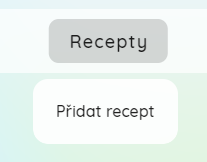
\includegraphics[width=\textwidth]{images/recipeo-hover}
    \caption{Schovaný odkaz na přidání receptu} \label{picture:recipeo:hover}
\end{figure}

\begin{figure}[H]
    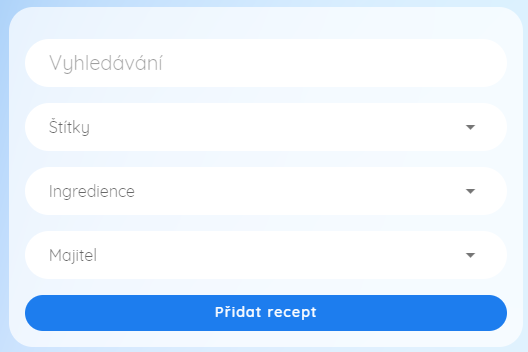
\includegraphics[width=\textwidth]{images/recipeo-add-button}
    \caption{Přidaný viditelný odkaz u seznamu receptů} \label{picture:recipeo:add-button}
\end{figure}

Další problém jsem našel hned s prvním respondentem. Bylo jím špatně navržené přepínání účtů. V horní liště byla zobrazena ikona s iniciály uživatele
popřípadě aktivní skupiny. Po najetí na ikonu se zobrazilo menu, kde si uživatel mohl vybrat mezi svým účtem a skupinami, ve kterých je členem. To
ovlivnilo i další místa v aplikaci jako zobrazení receptů nebo přidání receptu. To mohlo být pro uživatele, který o tomto nevěděl velmi matoucí, a
tak jsem se rozhodl prvky rozdělit a přidat do míst která ovládaly. Z lišty jsem tedy přesunul volbu uživatele k přidání receptu jako \emph{autocomplete}
a taktéž jsem učinil u filtrování receptů.

Dále jsme zjistili, že v některých situacích se nesprávně načítají data. Například při prvním spuštění aplikace a následovném přidání ingredience
se nenačetla její stránka. Nebo při přijmutí pozvánky do skupiny se nenačetly recepty, které skupina obsahuje.

Při přihlášení byl uživatel pouze přesměrován na úvodní stránku. To se všem respondentům zdálo jako nedostatečné upozornění na danou událost.
Přidal jsem tedy \emph{alert} z knihovny Vuetify, který by měl uživateli dát dostatečně najevo co se děje.

Jak jsem psal výše, na konci scénáře jsem s respondenty prošel aplikaci v mobilním zařízení. Dva z nich měli problém s akcí vrácení se na předchozí stránku,
tedy tlačítko zpět. Ovšem myslím si, že toto byl falešný poplach, způsobený tím, že test byl prováděn na počítači a mobilní zobrazení bylo pouze simulované.
Vzhledem k tomu, že se aplikace tváří jako nativní, uživatel by měl pro navigaci po aplikaci využívat prvky operačního systému, tedy šipku zpět v liště nebo
v novějších zařízeních gesto ze strany displeje.

\section{Vyhodnocení výsledků}

Vzhledem k nízkému počtu chyb v uživatelském rozhraní si dovolím říct, že \emph{frontend} aplikace testem použitelnosti prošel. Až na některé
skryté prvky, které jsem jednoduše naduplikoval na viditelnější místa, neměli testeři žádné problémy s navigací po aplikaci či využití
všech jejích funkcí. Design aplikace také všichni hodnotili pozitivně, což splňuje cíl, který jsem si stanovil při jeho návrhu. Tedy aby
se aplikace uživatelům líbila, působila moderně a byla srozumitelná.

Co se týče funkčnosti, zde to bylo horší a nejvíce problému se objevilo při stahování dat z databáze. Někdy nastaly situace, kde se správně
neaktualizovala data, a tak uživatel neměl přístup k veškerému obsahu. To ale nebyl problém spravit po nálezu míst, ve kterých se tyto nesrovnalosti
děly.

%! Author = Vojta
%! Date = 25.11.2021

\chapter{Možnosti aplikace v budoucnosti}

Během vývoje nastaly různé změny a některé funkce byly moc složité na implementaci nebo nebyly nutné v první verzi.
V této kapitole nastíním, jakým směrem by se aplikace mohla vydat.

\section{Interakce mezi uživateli}
V prototypu je možné pouze vytvořit skupinu, pozvat do ní ostatní uživatele a přidat do ní recepty. Původně jsem zamýšlel
i textovou komunikaci, ale nakonec jsme se s vedoucím shodli, že zatím není potřeba. Ovšem do budoucna by se mohla takováto
funkce hodit, v kombinaci s komentáři a hodnocením receptů. Poté by uživatelé mohli vybírat mezi veřejnými recepty podle
jejich kvality a sdílet své pocity či vychytávky.

Na to by se dalo navázat vytvořením profilů uživatelů. Na tomto profilu by uživatelé mohli přidávat příspěvky jako je tomu
například na Instagramu. Na této síti jsou populární krátká videa s recepty a tím pádem je zde potenciál pro případný % TODO: Citace
příliv uživatelů.

\section{Časovač}
U návrhu zobrazení receptu na mobilním zařízení jsem přidal časovač. V receptu by mohla být tlačítka u daných kroků, která
by spustila časovač na limit, který byl stanoven při vytvoření. Například by tedy po deseti minutách začal zvonit telefon, aby
uživatele upozornil na uvařené špagety. Seznam těchto měření by byl dostupný jako plovoucí tlačítko
v celé aplikaci a uživatel by tak k vaření potřeboval pouze mobilní zařízení.

\section{Verze FIT}
Kromě normálních receptů, by se dala aplikace přepnout do fitness módu, kde by zobrazovala pouze zdravé recepty. Nabídla by
také sledování kalorií, plány pro zlepšení stravy či jiné návrhy na úpravu jídelníčku.

\section{Pohodlí pro uživatele}
Jak jsem zmínil ve výsledcích kvalitativního průzkumu, uživatelé mají často problémy se zašpiněním dipleje na jejich zařízení při vaření.
Zabránit nepotřebného kontaktu se zařízením by mohlo pomoci například vynucení, aby obrazovka nezhasnula. Bylo by potřeba prozkoumat
\emph{Screen Wake Lock API}~\cite{ScreenWakeLockAPI} nebo nějaký plugin třetí strany.

\section{Propojení se službami Košík a Rohlík}
Tato práce měla být původně rozdělena na dvě, na frontend a na backend. Nakonec se nepodařilo sehnat studenta na backendovou část,
a tak jsem musel zpracovat fullstack aplikaci. Nezbyl tedy čas na implementaci doporučování, jednoduché přidání do košíku a dalších
funkcí napojené na služby Rohlíku a Košíku.

V budoucnu je ale jistě priorita tyto funkce zpřístupnit. Doporučení receptů by šlo založit na aktuálních slevách, daném ročním období či
uživatelově nákupní historii. S nákupy se pojí automatické přidání do spíže a sledování počtu surovin. Toto rozšíření spočívá v přidání
privátních ingrediencí, ke kterým si uživatel nebo skupina může přiřadit vlastní odkazy na zmíněné služby a počet kusů.

Zjednodušení nákupu by mohl zpřístupnit i plánovač. Uživatel by si naplánoval, co bude vařit další týden, poté označil dané dny a pomocí
jednoho tlačítka potřebné suroviny překlopil do nákupního košíku některé ze zmíněných služeb. Jako alternativu by mohl systém vygenerovat
nákupní lístek, který by v aplikaci přetrval a uživatel by jej mohl využít při nákupu v kamenném obchodě.

\section{Skupiny}
Při pozvání se nekontroluje žádný časový úsek či jiné ověření zda je pozvánka platná. Přidáním tokenu by se dala omezit doba platnosti
a tím zabránit nechtěnému šíření. Také stojí za zvážení operace nad členy skupiny. Tedy odebrání členů či smazání skupiny, které je zatím
nemožné.

%! Author = Vojta
%! Date = 25.11.2021

\chapter{Závěr}

% Shrnutí, možnosti do budoucna, nedoporučuje se používat emoční výrazy,
% nepoužívat obrázky, nadpisy, citace, nové myšlenky

Cílem práce bylo navržení a vytvoření webové aplikace, která usnadní manipulaci s recepty, surovinami či jejich nákupem.
Povedlo se naplnit většinu z původních požadavků, které stanovil vedoucí při zadávání a které jsem získal z průzkumu s potencionálními
uživateli. V první verzi aplikace, tedy prototypu, se dají využít základní funkce, které by měla aplikace poskytovat. Všechny tyto
funkce se dají v budoucnu rozšířit tak, aby splňovaly veškeré možnosti, které jsem v průběhu tvoření této práce objevil.

Ze začátku jsem se zabýval průzkumem konkurenčních řešení a kvalitativním průzkumem mezi potencionálními uživateli. Poté
jsem pokračoval návrhem papírových modelů a designem, což jsem spojil v jednu věc. Následovala volba technologií a tvorba
celého konceptu, jak vše bude fungovat. Mezitím jsem se domlouval s poskytovateli online nákupů surovin, zda by bylo možné
využít jejich služeb. Také jsem průběžně implementoval a přidával nové změny, které vzešly z problémů, na které jsem v průběhu
práce narazil. Nakonec jsem finální prototyp podrobil uživatelskému testování. Během tohoto testování jsem průběžně opravoval
chyby, na které testeři narazili.

Do budoucna se nabízí spousta možností okolo poskytnutých služeb od Rohlíku a Košíku. S tím také souvisí tvorba vlastního
API, které by aplikace pro tyto operace pravděpodobně potřebovala. Tím by se také osvobodila od různých limitů, které využívané
technologie s sebou přináší (potažmo verze, které jsou zdarma, po překročení limitů začíná být výhodnější platit pouze hosting
pro vlastní řešení). Ačkoliv při správné optimalizaci a chytrém využívání zdrojů, které momentální technologie nabízí, je možné
aplikaci rozšiřovat nad aktuální implementací.


% % Do not forget to include Introduction
%---------------------------------------------------------------
\chapter{Ut enim ad minim veniam}
%---------------------------------------------------------------
\setcounter{page}{1}

\begin{chapterabstract}
	\lipsum[1]
\end{chapterabstract}

\lipsum[2][1-4]{} [1]

\lipsum[4]

%---------------------------------------------------------------
\section{Ut enim ad minim veniam}
%---------------------------------------------------------------

\lipsum[6-7]

\begin{figure}
\centering
%\includegraphics[scale=0.4]{pic/index}
\resizebox{\textwidth}{!}{
\begin{tikzpicture}[level/.style={sibling distance=60mm/#1}]
\node [circle,draw] (z){$n$}
  child {node [circle,draw] (a) {$\frac{n}{2}$}
    child {node [circle,draw] (b) {$\frac{n}{2^2}$}
      child {node {$\vdots$}
        child {node [circle,draw] (d) {$\frac{n}{2^k}$}}
        child {node [circle,draw] (e) {$\frac{n}{2^k}$}}
      }
      child {node {$\vdots$}}
    }
    child {node [circle,draw] (g) {$\frac{n}{2^2}$}
      child {node {$\vdots$}}
      child {node {$\vdots$}}
    }
  }
  child {node [circle,draw] (j) {$\frac{n}{2}$}
    child {node [circle,draw] (k) {$\frac{n}{2^2}$}
      child {node {$\vdots$}}
      child {node {$\vdots$}}
    }
  child {node [circle,draw] (l) {$\frac{n}{2^2}$}
    child {node {$\vdots$}}
    child {node (c){$\vdots$}
      child {node [circle,draw] (o) {$\frac{n}{2^k}$}}
      child {node [circle,draw] (p) {$\frac{n}{2^k}$}
        child [grow=right] {node (q) {$=$} edge from parent[draw=none]
          child [grow=right] {node (q) {$O_{k = \lg n}(n)$} edge from parent[draw=none]
            child [grow=up] {node (r) {$\vdots$} edge from parent[draw=none]
              child [grow=up] {node (s) {$O_2(n)$} edge from parent[draw=none]
                child [grow=up] {node (t) {$O_1(n)$} edge from parent[draw=none]
                  child [grow=up] {node (u) {$O_0(n)$} edge from parent[draw=none]}
                }
              }
            }
            child [grow=down] {node (v) {$O(n \cdot \lg n)$}edge from parent[draw=none]}
          }
        }
      }
    }
  }
};
\path (a) -- (j) node [midway] {+};
\path (b) -- (g) node [midway] {+};
\path (k) -- (l) node [midway] {+};
\path (k) -- (g) node [midway] {+};
\path (d) -- (e) node [midway] {+};
\path (o) -- (p) node [midway] {+};
\path (o) -- (e) node (x) [midway] {$\cdots$}
  child [grow=down] {
    node (y) {$O\left(\displaystyle\sum_{i = 0}^k 2^i \cdot \frac{n}{2^i}\right)$}
    edge from parent[draw=none]
  };
\path (q) -- (r) node [midway] {+};
\path (s) -- (r) node [midway] {+};
\path (s) -- (t) node [midway] {+};
\path (s) -- (l) node [midway] {=};
\path (t) -- (u) node [midway] {+};
\path (z) -- (u) node [midway] {=};
\path (j) -- (t) node [midway] {=};
\path (y) -- (x) node [midway] {$\Downarrow$};
\path (v) -- (y)
  node (w) [midway] {$O\left(\displaystyle\sum_{i = 0}^k n\right) = O(k \cdot n)$};
\path (q) -- (v) node [midway] {=};
\path (e) -- (x) node [midway] {+};
\path (o) -- (x) node [midway] {+};
\path (y) -- (w) node [midway] {$=$};
\path (v) -- (w) node [midway] {$\Leftrightarrow$};
\path (r) -- (c) node [midway] {$\cdots$};
\end{tikzpicture}}
\caption{~Lorem ipsum dolor sit amet}\label{img:index}
\end{figure}

%---------------------------------------------------------------
\section{Ut enim ad minim veniam}
%---------------------------------------------------------------

\lipsum[2-4]

%---------------------------------------------------------------
\subsection{Ut enim ad minim veniam}
%---------------------------------------------------------------

Curabitur ligula sapien, pulvinar a vestibulum quis, facilisis vel sapien. Duis condimentum augue id magna semper rutrum. Aliquam ornare wisi eu metus. Fusce aliquam vestibulum ipsum. Vivamus ac leo pretium faucibus\ref{img:index}.

\begin{itemize}
    \item Ut enim ad minim veniam, quis nostrud
    \item Ut enim ad minim
    \item Ut enim ad minim veniam, quis
    \begin{itemize}
        \item Ut enim ad
        \item Ut enim ad
        \begin{itemize}
            \item Ut enim
            \item Ut enim
            \begin{itemize}
            \item Ut enim
            \item Ut enim
        \end{itemize}
        \end{itemize}
    \end{itemize}
\end{itemize}

\section{Class aptent taciti}

\lipsum[2]

\subsection{Class aptent taciti}

\lipsum[6-7]

\begin{enumerate}
    \item Ut enim ad minim veniam, quis nostrud
    \item Ut enim ad minim
    \item Ut enim ad minim veniam, quis
    \begin{enumerate}
        \item Ut enim ad
        \item Ut enim ad
        \begin{enumerate}
            \item Ut enim
            \item Ut enim
            \begin{enumerate}
            \item Ut enim
            \item Ut enim
        \end{enumerate}
        \end{enumerate}
    \end{enumerate}
\end{enumerate}


%---------------------------------------------------------------
\section{Ut enim ad minim veniam, quis nostrud}
%---------------------------------------------------------------

Ut enim ad minim veniam, quis nostrud exercitation ullamco laboris nisi ut aliquip ex ea commodo consequat. Nulla non arcu lacinia neque faucibus fringilla. Vestibulum erat nulla, ullamcorper nec, rutrum non, nonummy ac, erat. Aliquam erat volutpat. Proin pede metus, vulputate nec, fermentum fringilla, vehicula vitae, justo.\footnote{Ut enim ad minim veniam, quis nostrud exercitation.} Etiam dictum tincidunt diam. In laoreet, magna id viverra tincidunt, sem odio bibendum justo, vel imperdiet sapien wisi sed libero. Nulla est. Maecenas fermentum, sem in pharetra pellentesque, velit turpis volutpat ante, in pharetra metus odio a lectus. Duis aute irure dolor in reprehenderit in voluptate velit esse cillum dolore eu fugiat nulla pariatur.

%\begin{lstlisting}[caption={~Zbytečný kód},label=list:8-6,captionpos=t,float,abovecaptionskip=-\medskipamount,belowcaptionskip=\medskipamount,language=C]
%    #include<stdio.h>
%    #include<iostream>
%    // A comment
%    int main(void)
%    {
%        printf("Hello World\n");
%        return 0;
%    }
%\end{lstlisting}

%%%%%%%%%%%%%%%%%%%%%%%%%%%%%%%%%
% alternative using package minted for source highlighting
% package minted requires execution with `-shell-escape'
% e.g., `xelatex -shell-escape ctufit-thesis.tex'
\begin{listing}
\caption{Zbytečný kód}\label{list:8-6}
\begin{minted}{C}
    #include<stdio.h>
    #include<iostream>
    // A comment
    int main(void)
    {
        printf("Hello World\n");
        return 0;
    }
\end{minted}
\end{listing}
% %%%%%%%%%%%%%%%%%%%%%%%%%%%%%%%%%
Nullam feugiat, turpis at pulvinar vulputate, erat libero tristique tellus, nec bibendum odio risus sit amet ante. Aenean id metus id velit ullamcorper pulvinar. Fusce wisi. Integer lacinia. Aliquam id dolor. Pellentesque pretium lectus id turpis. Suspendisse sagittis ultrices augue. In laoreet, magna id viverra tincidunt, sem odio bibendum justo, vel imperdiet sapien wisi sed libero. Sed ac dolor sit amet purus malesuada congue. \cite{Crochemore2002}

Class aptent taciti sociosqu ad litora torquent per conubia nostra, per inceptos hymenaeos. Fusce suscipit libero eget elit. Etiam dui sem, fermentum vitae, sagittis id, malesuada in, quam. Aliquam id dolor. Curabitur bibendum justo non orci. Duis viverra diam non justo. Curabitur ligula sapien, pulvinar a vestibulum quis, facilisis vel sapien. Duis condimentum augue id magna semper rutrum. Aliquam ornare wisi eu metus. Fusce aliquam vestibulum ipsum. Vivamus ac leo pretium faucibus. \cite{Motwani2014}

%---------------------------------------------------------------
\subsection{Ut enim ad minim veniam, quis nostrud}
%---------------------------------------------------------------

Ut enim ad minim veniam, quis nostrud exercitation ullamco laboris nisi ut aliquip ex ea commodo consequat. Nulla non arcu lacinia neque faucibus fringilla. Vestibulum erat nulla, ullamcorper nec, rutrum non, nonummy ac, erat. Aliquam erat volutpat. Proin pede metus, vulputate nec, fermentum fringilla, vehicula vitae, justo. Etiam dictum tincidunt diam. In laoreet, magna id viverra tincidunt, sem odio bibendum justo. \cite{Sestakova2018}

\begin{table}\centering
\caption[Příklad tabulky]{~Zadávání matematiky}\label{tab:matematika}
\begin{tabular}{l|l|c|c}
	Typ		& Prostředí		& \LaTeX{}ovská zkratka	& \TeX{}ovská zkratka	\tabularnewline \hline
 	Text		& \verb|math|		& \verb|\(...\)|	& \verb|$...$|	\tabularnewline \hline
 	Displayed	& \verb|displaymath|	& \verb|\[...\]|	& \verb|$$...$$|	\tabularnewline
\end{tabular}
\end{table}


Nulla est. Maecenas fermentum, sem in pharetra pellentesque, velit turpis volutpat ante, in pharetra metus odio a lectus. Duis aute irure dolor in reprehenderit in voluptate velit esse cillum dolore eu fugiat nulla pariatur. Nullam feugiat, turpis at pulvinar vulputate, erat libero tristique tellus, nec bibendum odio risus sit amet ante. Aenean id metus id velit ullamcorper pulvinar.

\subsubsection{Class aptent taciti}

\begin{definition}[Optional label]
Class aptent taciti sociosqu ad litora torquent per conubia nostra, per inceptos hymenaeos. Fusce suscipit libero eget elit. Etiam dui sem, fermentum vitae, sagittis id, malesuada in, quam. Aliquam id dolor. Curabitur bibendum justo non orci.
\end{definition}

\begin{example}
Class aptent taciti sociosqu ad litora torquent per conubia nostra, per inceptos hymenaeos. Fusce suscipit libero eget elit. Etiam dui sem, fermentum vitae, sagittis id, malesuada in, quam. Aliquam id dolor. Curabitur bibendum justo non orci.
\end{example}

\begin{theorem}
Class aptent taciti sociosqu ad litora torquent per conubia nostra, per inceptos hymenaeos. Fusce suscipit libero eget elit. Etiam dui sem, fermentum vitae, sagittis id, malesuada in, quam. Aliquam id dolor. Curabitur bibendum justo non orci.
\end{theorem}

\begin{proof}
Fusce suscipit libero eget elit. Etiam dui sem, fermentum vitae, sagittis id, malesuada in, quam. Aliquam id dolor. Curabitur bibendum justo non orci.
\end{proof}

\begin{corollary}
Fusce suscipit libero eget elit. Etiam dui sem, fermentum vitae, sagittis id, malesuada in, quam. Aliquam id dolor. Curabitur bibendum justo non orci.
\end{corollary}

\begin{proposition}
Fusce suscipit libero eget elit. Etiam dui sem, fermentum vitae, sagittis id, malesuada in, quam. Aliquam id dolor. Curabitur bibendum justo non orci.
\end{proposition}

\begin{note}
Fusce suscipit libero eget elit. Etiam dui sem, fermentum vitae, sagittis id, malesuada in, quam. Aliquam id dolor. Curabitur bibendum justo non orci.
\end{note}

\begin{remark}
Fusce suscipit libero eget elit. Etiam dui sem, fermentum vitae, sagittis id, malesuada in, quam. Aliquam id dolor. Curabitur bibendum justo non orci.
\end{remark}

\begin{lemma}
Class aptent taciti sociosqu ad litora torquent per conubia nostra, per inceptos hymenaeos. Fusce suscipit libero eget elit. Etiam dui sem, fermentum vitae, sagittis id, malesuada in, quam. Aliquam id dolor. Curabitur bibendum justo non orci.
\end{lemma}

\lipsum[1-2]

\subsection{Class aptent taciti sociosqu}

\lipsum[4-5]

%---------------------------------------------------------------
\chapter{Lorem ipsum}
%---------------------------------------------------------------

\begin{chapterabstract}
	Lorem ipsum dolor sit amet, consectetuer adipiscing elit. Curabitur sagittis hendrerit ante. Class aptent taciti sociosqu ad litora torquent per conubia nostra, per inceptos hymenaeos. Cras pede libero, dapibus nec, pretium sit amet, tempor quis. Sed vel lectus. Donec odio tempus molestie, porttitor ut, iaculis quis, sem. Cras pede libero, dapibus nec, pretium sit amet, tempor quis. Sed vel lectus.
\end{chapterabstract}

Lorem ipsum dolor sit amet, consectetuer adipiscing elit. Curabitur sagittis hendrerit ante. Class aptent taciti sociosqu ad litora torquent per conubia nostra, per inceptos hymenaeos. Cras pede libero, dapibus nec, pretium sit amet, tempor quis. Sed vel lectus. Donec odio tempus molestie, porttitor ut, iaculis quis, sem. Suspendisse sagittis ultrices augue. Donec ipsum massa, ullamcorper in, auctor et, scelerisque sed, est. In sem justo, commodo ut, suscipit at, pharetra vitae, orci. Pellentesque pretium lectus id turpis. \cite{Kopka2004}

\section{Donec odio tempus molestie}

\lipsum[2] \cite{def:1, def:2}

\subsection{Class aptent taciti}

\lipsum[2-3]

\begin{description}
\item[Kapitola 1] Lorem ipsum dolor sit amet, consectetuer adipiscing elit. Curabitur sagittis hendrerit ante. Class aptent taciti sociosqu ad litora torquent per conubia nostra, per inceptos hymenaeos. Cras pede libero, dapibus nec, pretium sit amet, tempor quis.

\item[Kapitola 2] Lorem ipsum dolor sit amet, consectetuer adipiscing elit. Curabitur sagittis hendrerit ante. Class aptent taciti sociosqu ad litora torquent per conubia nostra, per inceptos hymenaeos. Cras pede libero, dapibus nec, pretium sit amet, tempor quis.

\item[Kapitola 3] Lorem ipsum dolor sit amet, consectetuer adipiscing elit. Curabitur sagittis hendrerit ante. Class aptent taciti sociosqu ad litora torquent per conubia nostra, per inceptos hymenaeos. Cras pede libero, dapibus nec, pretium sit amet, tempor quis.

\item[Kapitola 4] Lorem ipsum dolor sit amet, consectetuer adipiscing elit. Curabitur sagittis hendrerit ante. Class aptent taciti sociosqu ad litora torquent per conubia nostra, per inceptos hymenaeos. Cras pede libero, dapibus nec, pretium sit amet, tempor quis.
\end{description}

\lipsum[2]

\section{Lorem ipsum dolor sit amet}

\lipsum[3-5]
 % include `examples.tex' from `text/' subdirectory

\appendix\appendixinit % do not remove these two commands

\chapter{Nějaká příloha}


Sem přijde to, co nepatří do hlavní části.
 % include `appendix.tex' from `text/' subdirectory

\backmatter % do not remove this command

\printbibliography[title = {Zdroje}] % print out the BibLaTeX-generated bibliography list

%\chapter{Obsah přiloženého média}
% TODO: Odstranit?

	\dirtree{%
		.1 readme.txt\DTcomment{stručný popis obsahu média}.
		.1 exe\DTcomment{adresář se spustitelnou formou implementace}.
		.1 src.
		.2 impl\DTcomment{zdrojové kódy implementace}.
		.2 thesis\DTcomment{zdrojová forma práce ve formátu \LaTeX{}}.
		.1 text\DTcomment{text práce}.
		.2 thesis.pdf\DTcomment{text práce ve formátu PDF}.
	}
 % include `medium.tex' from `text/' subdirectory

\end{document}
